\documentclass[12pt]{report}

% Paquetes LaTeX y estilos globales
\input{etc/pkgs}
\input{etc/style}

%%%%%%%%%%%%%%%%%%%%%%%%%%%%%%%%%%%%%%%%%%%%%%%%%%%%%%%%%%%%%%%%%%%%%%%%%%%%%%%%%%%%%

% Variables para la portada
\setTitle{Olivaris - Plataforma de gestión colaborativa para el olivar} 
\setAuthor{Jorge Cano Melero} 
\setDegree{Grado en Ingeniería Informática} 
\setSupervisor{Juan Luis Jiménez Laredo} 
\setDepartment{Dpto. de Ingeniería de Computadores, Automática y Robótica}
\setMonth{junio} 
\setYear{2025/26} 

%%%%%%%%%%%%%%%%%%%%%%%%%%%%%%%%%%%%%%%%%%%%%%%%%%%%%%%%%%%%%%%%%%%%%%%%%%%%%%%%%%%%%

% Dedicatoria del trabajo
% Si no se desea incluir, comentar o borrar la línea siguiente para eliminar la página de dedicatoria
\setDedication{}

%%%%%%%%%%%%%%%%%%%%%%%%%%%%%%%%%%%%%%%%%%%%%%%%%%%%%%%%%%%%%%%%%%%%%%%%%%%%%%%%%%%%%

% Comienzo del documento
\begin{document}

    % Portada y secciones no numeradas
    \input{sections/00_portada}
    \chapter*{Agradecimientos}

Quiero agradecer este trabajo a mis padres, por ser los pilares fundamentales de mi vida, los que me han educado y han dado forma a mi personalidad.

Gracias por ayudarme a tomar una decisión tan importante para mí: cambiar el rumbo de mi vida y luchar por lo que uno quiere, independietemente de la edad,
afrontando la situación como si de un reto se tratara. Gracias a ellos puedo estar escribiendo estas palabras y estar presentando este Trabajo de Fin de Grado.

No puedo estar más orgulloso de todo lo que habéis hecho por mí y siempre estaré a vuestro lado.

Dar las gracias a otra persona tan importante como lo es mi hermano. Tu personalidad tan fuerte y trabajadora son un impulso para mí y un reflejo
donde mirarme. A pesar de ser el pequeño de la familia, demuestras una madurez increíble y siempre estas ayudando a los demás, demostrando ese amor y
compromiso que tienes. 

Me siento muy orgulloso de a persona en la que te estás convirtiendo y de lo que estás logrando, y que feliz me hace estar presente contigo para poder disfrutarlos 
juntos.

Y como no iba a poder agredecer desde lo más profundo de mi corazón este proyecto a mi pareja de vida, Carla. No sabría qué agradecerte en tan pocas líneas
después de todo lo que has hecho por mi y de todo el apoyo que me has dado desde hace más de 9 años. 

Gracias por ser enseñarme a comprender lo que significa la palabra amor, tratándolo como un sentimiento tan especial y que va más allá. Gracias por enseñarme a vivir 
más, por mirar siempre el lado positivo de las cosas y por agradecer cualquier gesto que nos da la vida.

Y por último, dar las gracias se queda corto al tutor de este Trabajo de Fin de Grado, Juan Luis Jiménez Laredo. Gracias por estar siempre disponible cuando lo he necestiado,
gracias por ayudarme en aquellos momentos del proyecto donde estaba perdido y no sabía cómo avanzar, gracias por tu positividad y tu empatía; sin ti este trabajo realizado no
tendría tanto significado para mí. Gracias por hacer el proceso enriquecedor, motivarme y confiar en mí.

A todas estas personas, gracias de nuevo por toda la ayuda que me habéis dado; habéis conseguido que disfrute del proceso y que el camino sea mucho más bonito. El orgullo que
siento por todos vosotros se queda corto.


    \newpage
    \thispagestyle{empty}
    \null
    \newpage
    \newpage
\begin{center}
    {\large \textbf{Olivaris - Plataforma de gestión colaborativa para el olivar}}
    
    \vspace{0.3cm}
    {\normalsize Jorge Cano Melero} 
    
    \vspace{0.3cm}
\end{center}

\vspace{0.5cm}

\textbf{Palabras clave:} Backend, API Rest

\vspace{0.5cm}

\textbf{Resumen:}

HACER RESUMEN
    \newpage
\begin{center}
    {\large \textbf{Olivaris - Plataforma de gestión colaborativa para el olivar}}

    \vspace{0.2cm}
    {\normalsize Jorge Cano Melero}

    \vspace{0.2cm}
\end{center}

\vspace{0.5cm}

\textbf{Keywords:} Commercial Farm Logbook, Agricultural Management, Backend, REST API, JWT, SIGPAC, Parcels, Phytosanitary Treatments.

\vspace{0.5cm}

\textbf{Abstract:}

This Final Degree Project addresses the design and implementation of Olivaris, a digital platform aimed at collaborative management of olive grove farms. The project arises in a context of increasing digitalization of 
the agricultural sector and regulatory evolution around the System of Information of Agricultural Farms, the Regional Registry of Agricultural Farms, and the Digital Farm Operation Logbook. Within this framework, Olivaris 
is presented as a tool to centralize the management of parcels, plots, users, authorized entities and agricultural activities, especially those related to the use of phytosanitary products.

The developed solution is based on a client-server architecture, with a backend that exposes a REST API, database persistence, authentication through JWT and role-based access control. The system allows registering and viewing 
parcels, managing activities associated with farms and modeling the relationship between farmers and authorized entities through access and management permissions.

Although the platform does not perform an effective integration with the official SIEX/REA services, its design has been developed taking into account the conceptual structure and information requirements associated with this 
framework, in order to facilitate a possible future integration. As a result, a functional and extensible prototype is obtained that contributes to the digitalization of olive grove management and serves as a basis for future 
improvements, such as offline functionality, advanced report generation or cross-platform access.
    \newpage \thispagestyle{empty} \mbox{} \newpage
\vspace{5cm}
\noindent\rule[-1ex]{\textwidth}{2pt}\\[4.5ex]

Yo, \textbf{Jorge Cano Melero}, alumno de la titulación Grado en Ingeniería Informática de la \textbf{Escuela Técnica Superior
de Ingenierías Informática y de Telecomunicación de la Universidad de Granada}, con DNI 77021264Z, autorizo la ubicación de la siguiente copia de mi Trabajo Fin de Grado en la biblioteca del centro para que pueda ser
consultada por las personas que lo deseen.

\vspace{6cm}

\noindent Fdo: Jorge Cano Melero

\vspace{2cm}

\begin{flushright}
% Fecha actual
Granada, \today
\end{flushright}

\newpage \thispagestyle{empty} \mbox{} \newpage

\newpage
\vspace{5cm}
\noindent\rule[-1ex]{\textwidth}{2pt}\\[4.5ex]

D. \textbf{Juan Luis Jiménez Laredo}, Profesor del Área de Arquitectura y Tecnología de Computadores
del Departamento de Ingeniería de Computadores, Automática y Robótica de la Universidad de Granada.

\vspace{0.5cm}

\textbf{Informa:}

\vspace{0.5cm}

Que el presente trabajo, titulado \textit{\textbf{ Olivaris - Plataforma de gestión colaborativa para el olivar }}, ha sido realizado bajo su supervisión por \textbf{Jorge Cano Melero}, y autorizo la defensa de dicho trabajo ante el tribunal que corresponda.

\vspace{0.5cm}

Y para que conste, expide y firma el presente informe en Granada, \today.

\vspace{1cm}

\textbf{El director:} Juan Luis Jiménez Laredo

\newpage \thispagestyle{empty} \mbox{} \newpage
    
    % Índice del documento y de figuras
    \begingroup
        % Los enlaces son normalmente azules, pero en los índices se configuran a negro para que no aparezca todo azul
        \hypersetup{linkcolor=black}
        \tableofcontents
        \listoffigures
        \listoftables
    \endgroup
    
    % Cambia el estilo de números de página de romanos a normal
    \clearpage\pagenumbering{arabic}
    
    % Capítulos del trabajo
    \chapter{Introducción}\label{cap:introduccion}

AÑADIR UNA INTRODUCCIÓN

\section{Estructura de la memoria}

La memoria va a estar divididad en los siguientes capítulos:

\begin{itemize}
    \item \textbf{Capítulo 1: Introducción}
    \newline
    En este capítulo se va a dar una breve introducción del producto que se va a desarrollar en el presente Trabajo de
    Fin de Grado. Además, se van a describir los distintos capítulos en los que se dividirá la memoria.

    \item \textbf{Capítulo 2: Estado del arte}
    \newline
    En este capítulo se realizará un análisis del contexto técnico y social del problema, así como un análisis de productos
    software relacionados, herramientas existentes para su desarrollo e implementación así como librerías.

    \item \textbf{Capítulo 3: Objetivos y Alcance}
    \newline
    Aunque los objetivos hayan sido mencionados anteriormente, aquí se entrará en más detalle describiendo tanto el
    objetivo general como los objetivos específicos del trabajo.

    \item \textbf{Capítulo 4: Metdología}
    \newline
    En este capítulo se explica cómo se ha trabajado durante el desarrollo del proyecto, abarcando tanto las metodologías
    de desarrollo como posibles intervenciones con personas usuarias (entrevistas, tests de usabilidad, etc).

    \item \textbf{Capítulo 5: Análisis y requisitos}
    

    \item \textbf{Capítulo 6: Diseño del sistema y arquitectura}
    \item \textbf{Capítulo 7: Implementación}
    \item \textbf{Capítulo 8: Evaluación y experimentación}
    \item \textbf{Capítulo 9: Conclusiones y trabajos futuros}
    \item \textbf{Capítulo 10: Referencias}
    \item \textbf{Capítulo 11: Glosario}
    \newline
    Este anexo va a recoger todos aquellos términos técnicos y de relevancia que se hayan usado en el presente documento,
    con la finalidad de aclarar aquellos conceptos que puedan ser confusos o no conocidos.
\end{itemize}
    \input{sections/02_Contexto_Estado}
    \chapter{Objetivos y alcance del proyecto}
    \chapter{Metodología}

En este capítulo se va a exponer cómo se ha desarrollado el proyecto en cuanto a organización y planificación de cada
una de las partes que lo han compuesto.

\section{Metodología de desarrollo}

Para la organización del proyecto se ha utilizado la metodología ágil \hyperlink{scrum}{\textbf{Scrum}} \cite{scrum}. 
Este tipo de metodología es muy útil debido a que permite ir realizando entregas del proyecto de forma iterativa y 
permite adaptarse a los cambios de forma rápida y eficiente.

A continuación se va a proceder a explicar en distintos apartados las piezas clave que componen el marco Scrum.

\subsection{Miembros del equipo Scrum}

Un equipo Scrum está formado por varios miembros, desempeñando cada uno un rol junto con unas responsabilidades.
Aunque normalmente la cantidad de miembros es reducida, pueden darse situaciones donde este número crezca considerablemente
porque así lo requiera el proyecto pero por lo general, los equipos de Scrum deben componerse de tres roles: el propietario
del producto (o \textit{Product Owner}), el \textit{Scrum Master} y el equipo de desarrollo.

En el proyecto, estos roles han sido asignados de la siguiente manera:

\begin{itemize}
    \item \textbf{Propieatrio del producto}
    \newline
    Este rol ha sido asignado tanto al tutor del TFG, el Dr. Juan Luis Jiménez 
    Laredo, así como al autor del presente proyecto. Se ha decidido así puesto que, entre ambos se ha ido dando forma
    a la propuesta: qué necesidades debía de cubrir el sistema, los requisitos funcionales  y las historias de usuario. 
    Asimismo, se encargaron de la priorización en cada iteración y de determinar cuando se consideraba cerrada una iteración,
    comprobando que el desarrollo fuese funcionando y incremental.

    \item \textbf{Scrum Master}
    \newline
    Este rol ha sido asignado al autor del proyecto, quien se ha encargado de asegurar el 
    cumplimiento de las prácticas Scrum mediante la orientación, eliminación de impedimentos, optimización del rendimiento 
    y entregas durante cada iteración.
    
    \item \textbf{Equipo de Desarrollo}
    \newline
    Este rol ha sido asignado al autor del proyecto debido a que ha sido el
    responsable de la ejecución técnica y el desarrollo del software.
\end{itemize}

\subsection{Artefactos de Scrum}

Los artefactos, dentro de la metodología Scrum, es información que el equipo utiliza para definir el trabajo que hay que
realizar para crear un producto. Hay tres tipos de artefactos: \textit{backlog} del producto, \textit{backlog} del sprint y
meta o incremento del sprint.

\begin{itemize}
    \item \textbf{Pila (\textit{backlog}) del Producto}
    \newline
    En este artefacto se agrupan todas las actividades en forma de lista que un equipo tiene que completar para crear el 
    producto. En este proyecto se ha utilizado la herramienta de GitHub Projects para crear un tablero donde se recojan 
    todas las actividades que se han planteado (historias de usuario, requisitos, mejoras y correcciones).

    \item \textbf{\textit{Backlog} del Sprint}
    \newline
    Esta sería la lista de elementos (historias de usuario y actividades) que el equipo de desarrollo ha seleccionado para
    realizar durante un sprint. Con la herramienta de GitHub Projects, además de poder tener una pila de producto con todas
    las actividades, se pueden agrupar las actividades por iteraciones / sprints y crear tableros que solo visualicen las 
    actividades relacionadas con ese sprint.

    \item \textbf{Meta del Sprint}
    \newline
    Este artefacto corresponde a la parte del producto que se obtiene al acabar una iteración. En este caso, cada vez 
    que se acaba la iteración, se obtiene una nueva funcionalidad que se añade al producto y que puede ser probada, con el fin
    de ir obteniendo algo ``tangible'' que el \textit{Product Owner} y el cliente pueda ver.
\end{itemize}

\subsection{Eventos de Scrum}

Con eventos de Scrum se va a referir a todas aquellas prácticas que son realizadas dentro del equipo Scrum de manera periódica,
englobando las ceremonias y reuniones que estos realizan en distintos momentos durante el desarrollo del producto.

Entre los eventos de Scrum, se encuentran los siguientes:

\begin{itemize}
    \item \textbf{Organización del Backlog}
    \newline
    Consiste en realizar una limpieza y actualización sobre la pila del producto, de manera que pueda estar lista para
    usarse por parte del equipo de desarrollo y de los miembros del equipo en cualquier momento. Esta labor es realizada
    por el \textit{Product Owner}.

    \item \textbf{Planificación de Sprints}
    \newline
    La planificación del sprint consiste en una reunión que realiza el equipo de desarrollo para planificar cual será
    el trabajo que se va a realizar durante el sprint. Esta reunión es diriga por el \textit{Scrum Master} y va a servir
    para ir añadiendo las historias de usuario o actividades importantes que se tengan que realizar, pasándolas del
    \textit{Product Backlog} al sprint específico.

    \item \textbf{Ejecución de Sprint}
    \newline
    Esta fase corresponde a la ejecución de todo lo planteado en el sprint, desarrollando e implementando todas aquellas
    tareas que han sido fijadas.

    \item \textbf{Reunión rápida}
    \newline
    Este tipo de ruenión se realiza al comienzo de la jornada de manera diaria. Son reuniones de corta duración donde se
    plantea lo que se va a realizar ese día y si hay algún obstáculo, de manera que todo el equipo trabaje en sintonía y
    se acerquen cada vez más a la consecución del sprint.

    \item \textbf{Revisión del Sprint}
    \newline
    La revisión del sprint consiste en una reunión en la que el equipo de desarrollo muestra a las partes interesadas del
    producto los elementos del backlog que están finalizados a través de una ``demo'', diciendo el \textit{Product Owner}
    si se publica o no el incremento.

    \item \textbf{Retrospectiva del Sprint}
    \newline
    Esta es la última reunión, donde el equipo se reúne para analizar qué cosas se han conseguido y han funcionado y cuales
    no, buscando de esta forma qué cosas deben mejorarse de cara a las próximas iteraciones.
\end{itemize}

\subsection{¿Por qué usar la metodología Scrum?}



\subsection{Adapatación de la metodología Scrum al proyecto}

Una vez explicadas todas las partes que componen la metodología Scrum, se va a proceder a explicar cómo esas partes han
sido adaptadas y tratadas en el presente proyecto.

Como se ha comentado anteriormente, se ha utilizado la herramienta de GitHub Projects \cite{githubProjects} para elaborar
el \textbf{\textit{Product Backlog}}, donde se han añadido todas las historias de usuario así como actividades necesarias
para poder desarrollar el software. A través de esta pila de producto se han ido organizando los diferentes sprints con 
las actividades necesarias para la realización de cada uno de ellos, ya que la herramienta de Projects permite crear distintas
vistas (cada una corresponde a un sprint) y asignar tareas del backlog a estas vistas. 

Tanto el Product Backlog como la planificación de cada uno de los sprints han sido llevados a cabo por el autor del proyecto, 
añadiendo toda la información (historias de usuario y tareas) que ha considerado necesaria para desarrollar el software 
junto con las recomendaciones del tutor del TFG (Dr. Juan Luis Jiménez Laredo) cuando ha sido requerido. Asimismo, la 
ejecución de cada sprint ha sido realizada por el autor del proyecto. En las imágenes ... se puede ver un ejemplo de cómo es
una historia de usurio y de cómo sería una sprint:

INSERTAR IMAGEN DE HISTORIA USUARIO

INSERTAR IMAGEN DE SPRINT 1

En cuanto a las reuniones realizadas durante todo el desarrollo del sistema, han sido tratas de la siguiente forma:

\begin{itemize}
    \item \textbf{Reunión diaria}: ha sido realizada por el autor del proyecto, revisando qué hizo el último día y planteando
    las siguientes tareas a desarrollar, teniendo en cuenta los plazos fijados y reorganizando tanto el sprint como
    el backlog en caso necesario. 

    \item \textbf{Revisión del sprint}: esta reunión ha sido realizada entre el tutor del TFG y el autor del proyecto al finalizar
    cada sprint. En esta reunión se han explicado las partes del software que han sido desarrolladas, se ha mostrado el funcionamiento
    del sistema y se ha debatido sobre posibles correcciones a realizar.

    \item \textbf{Reunión de retrospectiva}: ha sido realizada junto con el tutor del TFG y ha servido para tratar qué aspectos de lo
    realizado durante el sprint es mejorable y qué se podría añadir o contemplar para futuros sprints. También ha servido para fijar las 
    ideas de lo que iba a ser desarrollado en el próximo sprint y qué camino se iba a ir tomando.
\end{itemize}

\subsection{Sprints realizados}

Hablar de cada uno de los sprints realizados y del cronograma

\section{Presupuesto del proyecto}
    
    \chapter{Análisis y requisitos}\label{cap:especificación}

Antes de empezar con el desarrollo e implementación del sistema es necesario realizar una fase previa. En esta fase se 
van a extraer los requisitos que va a tener el sistema junto con las funcionalidades que tendrá. A 
continuación se va a explicar el proceso que se ha seguido.

\section{Recopilación de información}

Para recopilar información se ha recurrido a la realización de entrevistas, análisis de documentos y consultas a través
de correo electrónico con el personal adecuado.

\begin{itemize}
    \item \textbf{Entrevistas}
    \newline
    Se han realizado varias entrevistas con la finalidad de ajustar el sistema lo máximo posible a lo que se necesita
    o sería interesante que hubiese en el sector agrícola.

    \begin{itemize}
        \item \textbf{José Cobos Repiso - Agricultor de Cooperativa San Lorenzo de Zagra}
        \newline
        Con esta reunión se pudo ver cómo es el día a día de un agricultor que tiene varias fincas y cómo las gestiona.
        José mostró las distintas tablas que tiene creadas en Excel a través de las cuáles puede llevar un control exacto
        de qué actividad ha realizado en cada campaña y sobre qué finca en particular.
        Fueron varios los puntos planteados durante la reunión sobre qué podría tener la aplicación Olivaris. Entre
        ellos se destacaron:

        \begin{itemize}
            \item Funcionalidad de introducir un cuaderno de campo, siendo un punto muy interesante a tratar ya que el 
            próximo enero de 2027 va a ser obligatorio. Sobre esta funcionalidad se ha realizado un análisis más profundo
            que será comentado a continuación.
            \item Funcionalidad sobre control de costes y gastos, además de los pagos realizados a los empleados contratados.
            \item Funcionalidad sobre gestionar parcelas y las actividades realizadas en cada una de ellas, de manera que 
            se tenga una vista de todas las parcelas que son de su propiedad y se puedan gestionar las actividades de cada una
            de ellas. 
        \end{itemize}

        Gracias a este reunión se pudo obtener una aproximación de qué tipo de tablas se tendrían en la base de datos,
        cómo se podrían relacionar entre ellas y que funcionalidades tendría la aplicación.

        \item \textbf{Juan Luis Jiménez Laredo - Profesor titular de la ETSIIT y Director del presente TFG}
        \newline
        Las reuniones realizadas con Juan Luis han servido para llevar una revisión continua del desarrollo del proyecto,
        con la finalidad de saber qué requisitos funcionales tendrá el sistema y qué tareas hay que priorizar.
        Además, contando también con experiencia en el sector de la oliva, ha podido dar una visión del sistema más precisa,
        siendo esto de gran ayuda para definir cuáles son las funcionalidades más relevantes de la aplicación.

        Con la información extraída de la reunión realizada con José sobre el cuaderno de campo y con las conversaciones
        mantenidas con Juan Luis, se exploró la opción de introducir la funcionalidad del cuaderno de campo digital. 
        
        El \textbf{cuaderno de campo \cite{cuadernoCampo}} es una especie de cuaderno de bitácora que registra el uso 
        de productos químicos (fitosanitarios y fertilizantes) sobre una explotación con la finalidad de vigilar la 
        posible contaminación que pueda surgir derivada del abuso de estos productos. Este concepto está muy relacionado
        con el \textbf{Cuaderno Digital de Explotación Agrícola (CUE)}.

        Según la Conserjería de Agricultura, Pesca, Agua y Desarrollo Rural \cite{cueDigital}, el Cuaderno Digital de 
        Explotación Agrícola (o CUE digital), es la herramienta que se va a utilizar en España para anotar las 
        actividades que se realizan en una explotación agrícola, recogiendo las actividades fitosanitarias, de 
        fertilización o riegos aplicados. Para poder cumplimentar este CUE digital, es necesario que la explotación este
        previamente inscrita en REAFA (Registro Autonómico de Explotaciones Agrarias en Andalucía), ya que esta será la 
        fuente que proporcione la información de las parcelas y cultivos existentes.

        Este CUE digital, a diferencia del CUE de papel, obliga a que sea tratado desde medios electrónicos y que la
        información que lo cumplimente sea con los datos que la Administración tenga disponibles, procedentes del 
        Registro Autonómico de Explotaciones (REA).

        El aspecto que hace interesante la implementación de esta funcionalidad es que a partir del 1 de enero de 2027
        será obligatorio el uso del CUE digital para consignar la información de los tratamientos fitosanitarios. 
        
        A partir de este punto, se ha realizado una búsqueda de cómo acceder a la API que proporciona la Junta de 
        Andalucía para obtener los datos de una explotación y poder exportarlos al CUE digital. Para ello, primero es
        necesario dar de alta la ``empresa'' que va a desarrollar este proyecto en un portal junto con su certificado
        digital, estando aquí el primer problema: actualmente no hay constituida una empresa de desarrollo de software 
        particular, por lo que no hay certificado digital que se pueda utilizar para darse de alta y poder acceder a la
        API.

        Las soluciones buscadas han conllevado el envío de correos electrónicos a entidades que puedan suplir este problema
        y hacer de ``empresa de desarrollo''. Los correos enviados se van a comentar a continuación.
    \end{itemize}

    \item \textbf{Correos electrónicos}
    \newline
    Se han enviado correos electrónicos a las siguientes entidades, con la finalidad de buscar ayuda para dar de alta
    una empresa en el sistema y poder obtener el certificado digital que permita acceder a la API.

    \begin{itemize}
        \item \textbf{Nomia Energy}: empresa de Granada con la que se ha contactado para darla de alta en el registro
        como empresa desarrolladora del Cuaderno Digital de Explotación comercial. Con su certificado digital se podría
        acceder a la API pero finalmente no se llegó a un acuerdo y esta opción se descartó.

        \item \textbf{Trabajador de la Junta de Andalucía}: se mantuvieron conversaciones con Juan Carlos Martín Fuentes,
        trabajador de la Junta de Andalucía, para recoger qué requisitos son necesarios para registrarse como empresa de 
        desarrollo y sobre cómo tiene que ser el certificado digital, ya que se contempló la opción de trabajar con un 
        certificado ``autofirmado'' en el entorno de prepoducción (por no tener una empresa que proporcione el certificado), 
        pero finalmente esta opción se descartó porque no admiten certificados autofirmados, debido a la poca fiabilidad que
        tienen.        

        \item \textbf{Jefe de Seguridad de los Servicios Informáticos de la UGR}: se contactó con el Jefe de Seguridad
        para comentarle qué situación había, qué se quería realizar y cómo es el tipo de certificado digital que se 
        necesita para poder acceder a esta API. Se comentó las partes que deben incluir el certificado: parte pública 
        en formato .PEM, \hyperlink{certificadoTls}{\textit{TLS Web Client Authentiacion}} (clientAuth) y el 
        subdominio de la entidad o el CIF/NIF (el de la UGR en este caso), con la finalidad de saber si la UGR puede 
        gestionar un certificado con estas características y de esta forma poder acceder al sistema.
    \end{itemize}

    La funcionalidad del CUE digital es muy interesante pero ha tenido un problema: el proceso para extraer la información 
    es largo y lento (muchos correos electrónicos y tiempos de espera entre ellos), así como problemas derivados del uso de 
    un certificado digital que no se tiene, por lo que esta funcionalidad ha pasado a un segundo plano. El proyecto se ha 
    centrado en desarrollar el sistema con una base de datos y lógica de negocio propia que ``supla'' la falta de acceso a los
    endpoints de la API que se encargarían de realizar estas acciones.
\end{itemize}

\section{CUE comercial}

Durante esta fase de análisis, viendo la necesidad que va a haber a partir de enero del próximo año 2027 en facilitar un CUE comercial 
(aplicación software) a los titulares de una explotación, se ha orientado el desarrollo del sistema hacia este ámbito. Esta 
decisión ha causado que el sistema evolucione de un ERP clásico que se iba a desarrollar en un principio, a acotar el sistema 
a un diario de actividades que permita registrar su información en un CUE digital utilizando los datos suministrados por el usuario
y por la REA (en caso de poder acceder a la API).

A partir de este punto, el sistema a desarrollar debe poder acceder a la API o interfaz que suministran el \textbf{SIEX} (Sistema de Información
de Explotaciones Agrarias) para consumir sus endpoints, permitiendo obtener datos de la REA y exportar datos al CUE digital. Sin embargo, este 
proceso empezó siendo lento y tedioso, ya que requería un certificado que como se ha comentado antes, ha sido difícil de conseguir, por lo que se 
tomó la decisión de elaborar un sistema con una base de datos propia, que tenga las entidades necesarias para almacenar la información que podrían 
rellenar los datos del CUE digital. De esta manera, el sistema también estaría adaptado a una posible integración futura de la API, ya que sería añadir
el cliente de esta y que los datos sean enviados directamente a los servidores del REA y CUE que maneja el ministerio en vez de almacenarlos en las tablas.

Para obtener información sobre el CUE, se han accedido a los siguientes anexos principalmente:

\begin{itemize}
    \item \textbf{Anexo IX - Modelo de autorización de acceso a la información del REA y CUE:} este anexo se ha utilizado para saber qué permisos son
    los que cede un usuario que pertenece a una entidad habilitada sobre dicha entidad. Además de este, también se ha utilizado el anexo \textbf{Anexo VIII - 
    Modelo de Autorización de Representación} para investigar sobre los permisos.

    \item \textbf{Anexo VI - Interfaz Único Común:} este anexo se ha utilizado para comprender cómo funciona la interfaz de acceso o API. Como al final no 
    se pudo acceder a ella, la consulta a este anexo fue al inico del proyecto y sin entrar en detalle.

    \item \textbf{Anexo X - Registro de Autorizaciones para el uso de Aplicaciones Comerciales:} este anexo ha servido para comprender qué tipo de usuarios 
    van a interactuar con la aplicación y entre ellos, pudiendo distinguir entre tres: empresa desarrollador del software, entidad habilitada y titular de la
    explotación.

    \item \textbf{Anexo III - Registros de los tratamientos fitosanitarios y de fertilización:} este anexo se ha utilizado para investigar sobre qué datos de una
    explotación así como de una actividad fitosanitaria son utilizados para el cuaderno de explotación.
\end{itemize}

Otras fuentes que se visitaron para obtener más información fue el \textbf{Cuaderno de Explotación de la Junta de Andalucía}. En esta página se ha consultado 
información sobre el CUE Comercial (aplicación desarrollada), como por ejemplo: la fecha en la que será obligatorio el uso del CUE Digital para los agricultores 
en las actividades de tipo fitosanitario, o el proceso que tiene que seguir una empresa para darse de alta como CUE Comercial y poder acceder a la interfaz IUWS.

\section{Personas}

Una parte muy importante durante el análisis de un sistema son los usuarios finales que lo utilizan. Por ello, se han creado
personas ficticias que puedan representar al usuario que utiliza la aplicación, consiguiendo saber de esta manera cuáles son 
sus inquietudes y qué necesitan para poder realizar sus tareas correctamente.

En las imágenes \ref{fig:persona_1} y \ref{fig:persona_2} se muestran los tipos de usuarios que se han elaborado según las 
necesidades de la aplicación.

\begin{figure}[H]
    \centering
    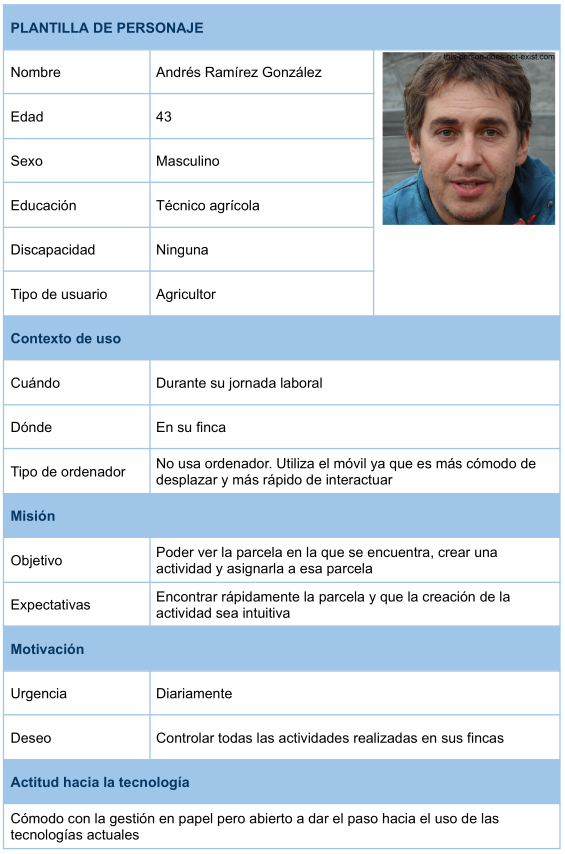
\includegraphics[width=0.8\textwidth]{figures/03_persona1.png}
    \caption{Persona 1: Agricultor}
    \label{fig:persona_1}
\end{figure}

\begin{figure}[H]
    \centering
    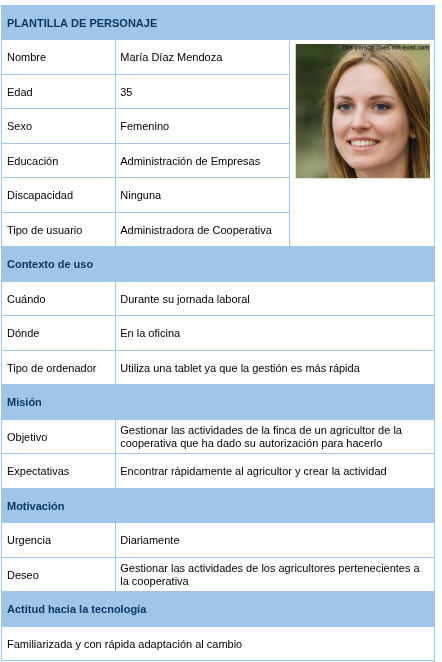
\includegraphics[width=0.8\textwidth]{figures/03_persona2.png}
    \caption{Persona 2: Administradora de la Cooperativa}
    \label{fig:persona_2}
\end{figure}

\section{Escenarios}

Una vez que han sido planteadas las personas, se pasa a describir los escenarios. Los escenarios son una descripción de
como el usuario utiliza el sistema para realizar una determinada tarea y lograr su objetivo. A través de esta técnica se
consigue ver de una forma más clara y cercana cómo debe de funcionar el sistema, pudiendo ayudar a encontrar y definir
requisitos funcionales.

Los escenarios planteados para las personas creadas en el apartado anterior son los siguientes:

\begin{itemize}
    \item \textbf{Primer escenario: Andrés Ramírez González (Agricultor)}
    \newline
    Andrés se encuentra realizando su jornada laboral en una de sus fincas y utiliza su móvil como herramienta principal 
    ya que necesita rapidez y se está moviendo constantemente.

    Andrés abre la aplicación y esta muestra un mapa con la geolocalización actual y las parcelas de su finca bien
    delimitadas. Procede a pulsar en una parcela y el sistema muestra información básica sobre la finca y un botón que le
    permite crear una actividad nueva asociada a esa parcela. Andrés selecciona esta opción y el sistema le envía a una 
    página que muestra un sencillo e intuitivo formulario que debe rellenar indicando el tipo de actividad que va a crear.

    Una vez guardada la información en el sistema, se muestra un mensaje de confirmación y se asocia automáticamente a la 
    parcela, pudiendo resivar Andrés el historial de actividades de esa finca en cualquier momento y controlando todo el 
    trabajo realizado en cualquier momento sin necesidad de papel.

    \begin{itemize}
        \item \textbf{Valor añadido}: identificación rápida de la parcela, creación de actividades de forma ágil y control
        centralizado de todas las tareas.
    \end{itemize}

    \item \textbf{Segundo escenario: María Díaz Mendoza (Administradora de Cooperativa)}
    \newline
    María se encuentra la oficina durante su jornada laboral, utilizando una tablet para gestionar de forma rápida y 
    eficiente tanto las fincas como actividades de los agricultores.

    María accede a la aplicación con su perfil de administradora de cooperativa y el sistema le muestra una lista con 
    todos los agricultores asociados que han autorizado la gestión de sus fincas, por lo que procede a seleccionar uno de ellos
    y el sistema le muestra una vista con todas las actividades asociadas a ese agricultor.

    María quiere añadir una nueva actividad por lo que pulsa sobre el botón que agrega una actividad. A continuación,
    se le presenta un formulario que debe de rellenar según la actividad a realizar.

    Una vez rellenado y guardado, el sistema la almacena automáticamente y la asocia a la parcela, quedando registrada para una
    consulta posterior tanto por María como por un agricultor. Este proceso se podrá repetir tantas veces como sea necesario con 
    distintos agricultores, asegurando una gestión centralizada y organizada.

    \begin{itemize}
        \item \textbf{Valor añadido}: gestión remota de varias fincas autorizadas, acceso rápido a las actividades y
        mejora de la coordinación y trazabilidad entre cooperativa y agricultores. 
    \end{itemize}
\end{itemize}

\section{Historias de Usuario}

Una \textbf{Historia de Usuario} \cite{historiaUsuario} es una descripción general e informal de una función de software escrita 
desde la persepectiva del usuario final o cliente. Su propósito es describir cómo un elemento de trabajo aporta un valor 
particular al cliente.

Son redactadas con un lenguaje sencillo y no técnico y consiguen con pocas palabras describir el resultado deseado. A partir de 
ellas se pueden establacer los requisitos funcionales del sistema y son añadidas a las iteraciones o \textit{sprints} dentro de 
la metodología ágil \hyperlink{scrum}{Scrum}.

Las historias de usuario son importantes ya que ayudan a los equipos de trabajo a centrarse en solucionar problemas para
usuarios reales, a que piensen de forma crítica y creativa sobre cómo lograr una meta de forma eficaz y ayudan a 
motivar al equipo ya que su resolución implica pequeños retos y victorias.

Para la realización de las Historias de Usuario del presente proyecto, la estructura utilizada ha sido la siguiente:

\textit{\textbf{Como} [tipo de usuario que realiza la acción], \textbf{quiero} [la acción que se quiere realizar] \textbf{para} 
[resultado obtenido].}

Además de la historia de usuario, se ha añadido el identificador de esa historia de usuario y un título identificativo.

Según los análisis realizados y la información obtenida, se han establecido las siguientes historias de usuario:

\begin{table}[H]
    \centering
    \begin{tabular}{|p{2cm}|p{4cm}|p{2cm}|p{4cm}|}
        \hline
        \textbf{ID} & HU-1 & \textbf{Nombre} & Inicio de sesión \\
        \hline
        \multicolumn{2}{|p{6cm}|}{\textbf{Descripción}} & \multicolumn{2}{p{6cm}|}{Como usuario, quiero iniciar sesión en la aplicación para acceder de forma segura a mis datos.} \\
        \hline
    \end{tabular}
    \caption{Historia de usuario HU-1}
    \label{tab:hu_1}
\end{table}

\begin{table}[H]
    \centering
    \begin{tabular}{|p{2cm}|p{4cm}|p{2cm}|p{4cm}|}
        \hline
        \textbf{ID} & HU-2 & \textbf{Nombre} & Sesión segura \\
        \hline
        \multicolumn{2}{|p{6cm}|}{\textbf{Descripción}} & \multicolumn{2}{p{6cm}|}{Como usuario, quiero que mi sesión sea segura para evitar accesos no autorizados.} \\
        \hline
    \end{tabular}
    \caption{Historia de usuario HU-2}
    \label{tab:hu_2}
\end{table}

\begin{table}[H]
    \centering
    \begin{tabular}{|p{2cm}|p{4cm}|p{2cm}|p{4cm}|}
        \hline
        \textbf{ID} & HU-3 & \textbf{Nombre} & Asignación de roles \\
        \hline
        \multicolumn{2}{|p{6cm}|}{\textbf{Descripción}} & \multicolumn{2}{p{6cm}|}{Como administrador, quiero asignar roles a los usuarios para controlar qué puede hacer cada uno.} \\
        \hline
    \end{tabular}
    \caption{Historia de usuario HU-3}
    \label{tab:hu_3}
\end{table}

\begin{table}[H]
    \centering
    \begin{tabular}{|p{2cm}|p{4cm}|p{2cm}|p{4cm}|}
        \hline
        \textbf{ID} & HU-4 & \textbf{Nombre} & Control de funcionalidad según rol \\
        \hline
        \multicolumn{2}{|p{6cm}|}{\textbf{Descripción}} & \multicolumn{2}{p{6cm}|}{Como administrador, quiero que el sistema controle el acceso a cada funcionalidad según el rol para evitar manipulación indeseada de datos.} \\
        \hline
    \end{tabular}
    \caption{Historia de usuario HU-4}
    \label{tab:hu_4}
\end{table}

\begin{table}[H]
    \centering
    \begin{tabular}{|p{2cm}|p{4cm}|p{2cm}|p{4cm}|}
        \hline
        \textbf{ID} & HU-5 & \textbf{Nombre} & Registro de entidades habilitadas \\
        \hline
        \multicolumn{2}{|p{6cm}|}{\textbf{Descripción}} & \multicolumn{2}{p{6cm}|}{Como usuario quiero registrar una entidad en el sistema para que se puedan gestionar los datos de los usuarios que pertenezcan a ella.} \\
        \hline
    \end{tabular}
    \caption{Historia de usuario HU-5}
    \label{tab:hu_5}
\end{table}

\begin{table}[H]
    \centering
    \begin{tabular}{|p{2cm}|p{4cm}|p{2cm}|p{4cm}|}
        \hline
        \textbf{ID} & HU-6 & \textbf{Nombre} & Control de actividades \\
        \hline
        \multicolumn{2}{|p{6cm}|}{\textbf{Descripción}} & \multicolumn{2}{p{6cm}|}{Como entidad habilitada, quiero gestionar las fincas y sus actividades para que el agricultor no tenga que realizar estas tareas.} \\
        \hline
    \end{tabular}
    \caption{Historia de usuario HU-6}
    \label{tab:hu_6}
\end{table}

\begin{table}[H]
    \centering
    \begin{tabular}{|p{2cm}|p{4cm}|p{2cm}|p{4cm}|}
        \hline
        \textbf{ID} & HU-7 & \textbf{Nombre} & Gestión de parcelas \\
        \hline
        \multicolumn{2}{|p{6cm}|}{\textbf{Descripción}} & \multicolumn{2}{p{6cm}|}{Como agricultor, quiero registrar una parcela con sus datos para poder gestionarla correctamente.} \\
        \hline
    \end{tabular}
    \caption{Historia de usuario HU-7}
    \label{tab:hu_7}
\end{table}

\begin{table}[H]
    \centering
    \begin{tabular}{|p{2cm}|p{4cm}|p{2cm}|p{4cm}|}
        \hline
        \textbf{ID} & HU-8 & \textbf{Nombre} & Registro de actividades \\
        \hline
        \multicolumn{2}{|p{6cm}|}{\textbf{Descripción}} & \multicolumn{2}{p{6cm}|}{Como agricultor, quiero registrar una actividad diaria para llevar un control centralizado.} \\
        \hline
    \end{tabular}
    \caption{Historia de usuario HU-8}
    \label{tab:hu_8}
\end{table}

\begin{table}[H]
    \centering
    \begin{tabular}{|p{2cm}|p{4cm}|p{2cm}|p{4cm}|}
        \hline
        \textbf{ID} & HU-9 & \textbf{Nombre} & Registro de actividad fitosanitaria \\
        \hline
        \multicolumn{2}{|p{6cm}|}{\textbf{Descripción}} & \multicolumn{2}{p{6cm}|}{Como agricultor, quiero registrar un tratamiento fitosanitario para cumplir la normativa.} \\
        \hline
    \end{tabular}
    \caption{Historia de usuario HU-9}
    \label{tab:hu_9}
\end{table}

\begin{table}[H]
    \centering
    \begin{tabular}{|p{2cm}|p{4cm}|p{2cm}|p{4cm}|}
        \hline
        \textbf{ID} & HU-10 & \textbf{Nombre} & Registro de actividad futura o planificada \\
        \hline
        \multicolumn{2}{|p{6cm}|}{\textbf{Descripción}} & \multicolumn{2}{p{6cm}|}{Como agricultor, quiero planificar actividades futuras para organizar el trabajo de la campaña.} \\
        \hline
    \end{tabular}
    \caption{Historia de usuario HU-10}
    \label{tab:hu_10}
\end{table}

\begin{table}[H]
    \centering
    \begin{tabular}{|p{2cm}|p{4cm}|p{2cm}|p{4cm}|}
        \hline
        \textbf{ID} & HU-11 & \textbf{Nombre} & Modificación de actividad \\
        \hline
        \multicolumn{2}{|p{6cm}|}{\textbf{Descripción}} & \multicolumn{2}{p{6cm}|}{Como agricultor, quiero modificar una actividad almacenada para corregir datos o marcarla como realizada.} \\
        \hline
    \end{tabular}
    \caption{Historia de usuario HU-11}
    \label{tab:hu_11}
\end{table}

\begin{table}[H]
    \centering
    \begin{tabular}{|p{2cm}|p{4cm}|p{2cm}|p{4cm}|}
        \hline
        \textbf{ID} & HU-12 & \textbf{Nombre} & Eliminación de actividad \\
        \hline
        \multicolumn{2}{|p{6cm}|}{\textbf{Descripción}} & \multicolumn{2}{p{6cm}|}{Como agricultor, quiero eliminar una actividad para no tenerla guardada en el sistema.} \\
        \hline
    \end{tabular}
    \caption{Historia de usuario HU-12}
    \label{tab:hu_12}
\end{table}

\begin{table}[H]
    \centering
    \begin{tabular}{|p{2cm}|p{4cm}|p{2cm}|p{4cm}|}
        \hline
        \textbf{ID} & HU-13 & \textbf{Nombre} & Control de usuarios \\
        \hline
        \multicolumn{2}{|p{6cm}|}{\textbf{Descripción}} & \multicolumn{2}{p{6cm}|}{Como administrador, quiero obtener los usuarios registrados en el sistema para llevar un control de quien está registrado.} \\
        \hline
    \end{tabular}
    \caption{Historia de usuario HU-13}
    \label{tab:hu_13}
\end{table}

\begin{table}[H]
    \centering
    \begin{tabular}{|p{2cm}|p{4cm}|p{2cm}|p{4cm}|}
        \hline
        \textbf{ID} & HU-14 & \textbf{Nombre} & Consulta de parcela \\
        \hline
        \multicolumn{2}{|p{6cm}|}{\textbf{Descripción}} & \multicolumn{2}{p{6cm}|}{Como agricultor, quiero consultar mis parcelas, para obtener información sobre ellas.} \\
        \hline
    \end{tabular}
    \caption{Historia de usuario HU-14}
    \label{tab:hu_14}
\end{table}

\begin{table}[H]
    \centering
    \begin{tabular}{|p{2cm}|p{4cm}|p{2cm}|p{4cm}|}
        \hline
        \textbf{ID} & HU-15 & \textbf{Nombre} & Consulta de actividades \\
        \hline
        \multicolumn{2}{|p{6cm}|}{\textbf{Descripción}} & \multicolumn{2}{p{6cm}|}{Como agricultor, quiero consultar el historial de actividades de un usuario para saber todo lo que ha realizado.} \\
        \hline
    \end{tabular}
    \caption{Historia de usuario HU-15}
    \label{tab:hu_15}
\end{table}

\begin{table}[H]
    \centering
    \begin{tabular}{|p{2cm}|p{4cm}|p{2cm}|p{4cm}|}
        \hline
        \textbf{ID} & HU-16 & \textbf{Nombre} & Visualización de parcelas en un mapa \\
        \hline
        \multicolumn{2}{|p{6cm}|}{\textbf{Descripción}} & \multicolumn{2}{p{6cm}|}{Como agricultor, quiero visualizar mis parcelas en un mapa para conocer rápidamente el estado de las tareas.} \\
        \hline
    \end{tabular}
    \caption{Historia de usuario HU-16}
    \label{tab:hu_16}
\end{table}

\begin{table}[H]
    \centering
    \begin{tabular}{|p{2cm}|p{4cm}|p{2cm}|p{4cm}|}
        \hline
        \textbf{ID} & HU-17 & \textbf{Nombre} & Cierre de sesión \\
        \hline
        \multicolumn{2}{|p{6cm}|}{\textbf{Descripción}} & \multicolumn{2}{p{6cm}|}{Como usuario, quiero cerrar sesión para proteger mis datos cuando dejo de usar la aplicación.} \\
        \hline
    \end{tabular}
    \caption{Historia de usuario HU-17}
    \label{tab:hu_17}
\end{table}

\begin{table}[H]
    \centering
    \begin{tabular}{|p{2cm}|p{4cm}|p{2cm}|p{4cm}|}
        \hline
        \textbf{ID} & HU-18 & \textbf{Nombre} & Registro de actividades \\
        \hline
        \multicolumn{2}{|p{6cm}|}{\textbf{Descripción}} & \multicolumn{2}{p{6cm}|}{Como agricultor, quiero registrar una actividad directamente desde el mapa para agilizar el trabajo en campo.} \\
        \hline
    \end{tabular}
    \caption{Historia de usuario HU-18}
    \label{tab:hu_18}
\end{table}

\section{Criterios de aceptación}

Las historias de usuario definidas tienen unos criterios de aceptación asociados que establecen cuando una historia de usuario ha sido
completada. Los criterios de aceptación para cada historia de usuario son los siguientes:

\begin{itemize}
    \item \textbf{HU-01}
    \begin{itemize}
        \item Dado que introduzco usuario/email y contraseña correctos, cuando inicio sesión, entonces accedo a la aplicación.
        \item Dado que no he confirmado mi registro, cuando inicio sesión, el sistema no me lo permite.
        \item Dado que introduzco credenciales incorrectas, cuando intento iniciar sesión, entonces el sistema muestra un mensaje de error.
        \item Dado que no estoy autenticado, cuando intento acceder a una funcionalidad protegida, el sistema no me lo permite.
    \end{itemize}
\end{itemize}

\begin{itemize}
    \item \textbf{HU-02}
    \begin{itemize}
        \item Dado que inicio sesión, cuando pasa el tiempo de inactividad configurado, entonces la sesión expira.
        \item Dado que la sesión expira, cuando intento continuar, entonces debo volver a autenticarme.
    \end{itemize}
\end{itemize}

\begin{itemize}
    \item \textbf{HU-03}
    \begin{itemize}
        \item Dado que un usuario tiene un rol asignado, cuando accede al sistema, entonces solo puede realizar lo permitido.
    \end{itemize}
\end{itemize}

\begin{itemize}
    \item \textbf{HU-04}
    \begin{itemize}
        \item Dado que intento realizar una acción no permitida en base a mi rol, entonces el sistema lo bloquea.
    \end{itemize}
\end{itemize}

\begin{itemize}
    \item \textbf{HU-05}
    \begin{itemize}
        \item Un usuario con rol de administrador puede crear una entidad habilitada en el sistema.
        \item El sistema impedirá que un usuario con otro rol quiera registrar una entidad.
        \item Los campos de nombre, NIF y correo electrónico son obligatorios; sin ellos no se podrá crear la entidad.
    \end{itemize}
\end{itemize}

\begin{itemize}
    \item \textbf{HU-06}
    \begin{itemize}
        \item El sistema no permite que un usuario con rol administrador dentro de una entidad pueda manipular datos de usuarios que no le han dado permiso.
        \item El sistema no permite que un usuario pueda gestionar datos o usuarios de otras entidades a las que no pertenece.
        \item Un usuario que pertenece a una entidad con rol administrador podrá gestionar las actividades de otro usuario que haya otorgado permisos dentro 
        de la misma entidad.
    \end{itemize}
\end{itemize}

\begin{itemize}
    \item \textbf{HU-07}
    \begin{itemize}
        \item Dado que introduzco los datos válidos de una parcela, cuando la guardo, entonces la parcela queda registrada en el sistema.
        \item Dado que la parcela tiene recintos, cuando se guarda la parcela, entonces los recintos quedan almacenados y vinculados a la parcela.
        \item Dado que faltan datos obligatorios de la parcela, cuando intento guardarla, entonces el sistema muestra un error indicando los campos inválidos.
        \item Dado que existen recintos con datos inválidos o incompletos, cuando intento guardar la parcela, entonces el sistema muestra un error.
    \end{itemize}
\end{itemize}

\begin{itemize}
    \item \textbf{HU-08}
    \begin{itemize}
        \item Dado que introduzco datos válidos de una actividad, cuando la guardo, entonces la actividad queda registrada en el sistema.
        \item Dado que la actividad tiene estado ``Completada'', cuando introduzco una fecha futura, entonces el sistema muestra un error.
        \item Dado que falta alguno de los campos obligatorios (fecha, campaña, parcela/recinto o tipo de actividad), cuando intento guardar, entonces el 
        sistema muestra un error indicando los campos inválidos.
        \item Dado que la parcela o recinto no existe, cuando intento registrar la actividad, entonces el sistema muestra un error.
        \item Dado que el usuario es admin dentro de una entidad, cuando registra una actividad para otro usuario de su entidad con permisos, entonces la 
        actividad se guarda correctamente.
        \item Dado que el usuario es ``agricultor'' o ``administrador'' y no pertenecen a ninguna entidad con rol ``agricultor'', cuando registra una actividad, 
        entonces solo puede hacerlo para sí mismo.
    \end{itemize}
\end{itemize}

\begin{itemize}
    \item \textbf{HU-09}
    \begin{itemize}
        \item Dado que selecciono el tipo de actividad ``fitosanitaria'', cuando accedo al formulario de registro, entonces el sistema solicita los campos 
        necesarios como dosis, NIF del aplicador, fecha y tipo de cultivo.
        \item Dado que introduzco todos los datos válidos de un tratamiento fitosanitario, cuando guardo la actividad, entonces el tratamiento queda registrado 
        en el sistema y asociado a la actividad.
        \item Dado que falta alguno de los campos obligatorios cuando intento guardar, entonces el sistema muestra un error indicando los campos inválidos.
        \item Dado que registro un tratamiento fitosanitario válido, cuando se guarda la actividad, entonces se almacena en la tabla de actividades y en la 
        tabla específica de tratamientos.
    \end{itemize}
\end{itemize}

\begin{itemize}
    \item \textbf{HU-10}
    \begin{itemize}
        \item Dado que introduzco los datos válidos de una actividad con fecha futura, cuando la guardo, entonces la actividad queda registrada en el sistema 
        como ``Planificada''.
        \item Dado que intento registrar una actividad planificada, cuando introduzco una fecha pasada, entonces el sistema muestra un error.
        \item Dado que no se ha insertado una campaña, cuando intento guardar la actividad, entonces el sistema muestra un error. 
    \end{itemize}
\end{itemize}

\begin{itemize}
    \item \textbf{HU-11}
    \begin{itemize}
        \item Dado que existe una actividad registrada, cuando modifico sus datos con valores válidos y guardo, entonces la actividad se actualiza correctamente 
        en el sistema.
        \item Dado que falta algún campo obligatorio tras la modificación, cuando intento guardar los cambios, entonces el sistema muestra un error.
        \item Dado que se modifica el estado de una actividad ``completada'' a ``planificada'', el sistema muestra un error. 
    \end{itemize}
\end{itemize}

\begin{itemize}
    \item \textbf{HU-12}
    \begin{itemize}
        \item Dado que elimino una actividad, si esta existe, entonces desaparece.
        \item Dado que la actividad contenía datos en tablas específicas, entonces los datos asociados se eliminan o recalculan.
    \end{itemize}
\end{itemize}

\begin{itemize}
    \item \textbf{HU-13}
    \begin{itemize}
        \item Dado que el usuario tiene rol ``administrador'', cuando accede al listado de usuarios, entonces el sistema muestra 
        todos los usuarios registrados.
        \item Dado que el usuario no tiene rol ``administrador'', cuando intenta acceder al listado de usuarios, entonces el 
        sistema deniega el acceso.
        \item Dado que accedo al listado de usuarios, cuando se muestran los resultados, entonces veo los datos básicos de 
        cada usuario (nombre, email, rol y estado).
    \end{itemize}
\end{itemize}

\begin{itemize}
    \item \textbf{HU-14}
    \begin{itemize}
        \item Dado que el usuario existe en el sistema, puede acceder a la información de sus parcelas.
        \item Dado que el usuario tiene la parcela asignada, entonces se muestra la información de ella.
    \end{itemize}
\end{itemize}

\begin{itemize}
    \item \textbf{HU-15}
    \begin{itemize}
        \item Dado que el historial de actividades es de un usuario distinto del que las quiere obtener, 
        en caso de no tener rol de administrador dentro de la misma entidad el sistema lo impedirá.
    \end{itemize}
\end{itemize}

\begin{itemize}
    \item \textbf{HU-16}
    \begin{itemize}
        \item Dado que el usuario existe, el sistema obtiene las parcelas asignadas a el y las dibuja 
        sobre un mapa.
    \end{itemize}
\end{itemize}

\begin{itemize}
    \item \textbf{HU-17}
    \begin{itemize}
        \item Dado que he iniciado sesión en el sistema, cuando cierro sesión, los tokens que me permiten
        el acceso son eliminados y no puedo acceder al sistema.
        \item Dado que la sesión ha sido cerrada, hay que iniciar sesión de nuevo para poder acceder al sistema.
    \end{itemize}
\end{itemize}

\begin{itemize}
    \item \textbf{HU-18}
    \begin{itemize}
        \item Dado que la parcela y el recinto aparece dibujado en el mapa, cuando el usuario clicka en ella,
        aparece un enlace al formulario de registro.
        \item Dado que se registra correctamente la actividad, queda almacenada en las tablas del sistema.
    \end{itemize}
\end{itemize}

\section{Requisitos funcionales}

Los requisitos funcionales sirven para indicar qué funciones tiene el sistema y qué debe hacer. A partir 
de las historias de usuario se han extraído los siguientes requisitos funcionales agrupados por áreas. 
La estructura es del tipo \textit{RF-[ID de HU].XX}.

\subsection{Autenticación y autorización}

\begin{itemize}
    \item \textbf{RF-01.1)} El sistema debe permitir autenticación mediante usuario/email y contraseña.
    \item \textbf{RF-01.2)} El sistema debe validar las credenciales contra la base de datos.
    \item \textbf{RF-01.3)} El sistema debe iniciar una sesión de usuario tras autenticación correcta.
    \item \textbf{RF-01.4)} El sistema debe impedir el acceso a usuarios no autenticados.
    \item \textbf{RF-02.1)} El sistema debe gestionar expiración de sesiones o tokens.
    \item \textbf{RF-02.2)} El sistema debe invalidar sesiones antiguas automáticamente.
    \item \textbf{RF-02.3)} El sistema debe proteger endpoints con autenticación obligatoria.
    \item \textbf{RF-03.1)} El sistema debe soportar al menos los roles: administrador, entidad habilitada (cooperativa), agricultor.
    \item \textbf{RF-03.2)} El sistema debe evaluar permisos en función del rol del usuario.
    \item \textbf{RF-03.3)} El sistema debe ocultar o deshabilitar funcionalidades no autorizadas.
    \item \textbf{RF-04.1)} El sistema debe validar permisos antes de ejecutar cualquier acción.
    \item \textbf{RF-04.2)} El sistema debe impedir operaciones no autorizadas a nivel de backend.
    \item \textbf{RF-17.1)} El sistema debe eliminar los tokens guardados del usuario para evitar futuras peticiones.
    \item \textbf{RF-17.2)} El sistema debe mostrar la página de inicio de sesión en caso de haber cerrido la sesión.
\end{itemize}

\subsection{Entidades habilitadas}

\begin{itemize}
    \item \textbf{RF-05.1)} El sistema debe permitir registrar una entidad habilitada en el sistema si los campos son correctos.
    \item \textbf{RF-05.2)} El sistema debe impedir el registro de una entidad a un usuario con rol distinto de administrador.
    \item \textbf{RF-06.1)} Se crea una relación entre el usuario y la entidad habilitada con un rol y los permisos que cede a la entidad.
    \item \textbf{RF-06.2)} Los roles posibles dentro de una entidad son: agricultor (farmer) y admin (administrador).
    \item \textbf{RF-06.3)} Las actividades pueden ser manipuladas por el usuario que tenga el rol admin dentro de la entidad y sobre los
    usuarios que pertenezcan a esa entidad.
    \item \textbf{RF-06.4)} Si usuario agricultor es vinculado con una entidad, cede directamente todos sus permisos a la entidad. 
\end{itemize}

\subsection{Parcelas y recintos}

\begin{itemize}
    \item \textbf{RF-07.1)} El sistema debe permitir al usuario registrar parcelas.
    \item \textbf{RF-07.2)} El sistema debe validar que los campos obligatorios de la parcela sean correctos antes de su creación.
    \item \textbf{RF-07.3)} El sistema debe mostrar un error si la validación de la parcela falla.
    \item \textbf{RF-07.4)} El sistema debe consumir la API de SIGPAC para obtener los datos de parcelas y recintos (códigos y geometrías/polígonos).
    \item \textbf{RF-07.5)} El sistema debe almacenar la parcela en la base de datos.
    \item \textbf{RF-07.6)} El sistema debe almacenar los recintos asociados a una parcela, en caso de que existan.
    \item \textbf{RF-07.7)} El sistema debe vincular los recintos con su parcela correspondiente.
    \item \textbf{RF-14.1)} El sistema debe devolver la información de una parcela vinculada a un usuario específico.
    \item \textbf{RF-16.1)} El sistema debe devolver una lista con la información de una parcela junto con la geometría para el propio usuario.
    \item \textbf{RF-16.2)} El sistema debe validar que el usuario existe.
    \item \textbf{RF-18.1)} El sistema debe mostrar un enlace que lleve al formulario de crear una actividad al clickar sobre un recinto del mapa.
\end{itemize}

\subsection{Actividades}

\begin{itemize}
    \item \textbf{RF-08.1)} El sistema debe permitir registrar actividades.
    \item \textbf{RF-08.2)} El sistema debe permitir registrar actividades con estado ``Planificada'' o ``Completada''.
    \item \textbf{RF-08.3)} El sistema debe impedir registrar actividades con fecha futura si el estado es ``Realizada''.
    \item \textbf{RF-08.4)} El sistema debe validar que la parcela o recinto asociado exista.
    \item \textbf{RF-08.5)} El sistema debe validar que la actividad esté asociada a una campaña.
    \item \textbf{RF-08.6)} El sistema debe validar que el tipo de actividad pertenezca al catálogo permitido.
    \item \textbf{RF-08.7)} El sistema debe validar que los campos obligatorios (fecha, parcela/recinto, campaña, tipo de actividad) estén presentes.
    \item \textbf{RF-08.8)} El sistema debe impedir guardar la actividad si falla alguna validación.
    \item \textbf{RF-08.9)} El sistema debe almacenar la actividad en el sistema actualizando automáticamente las tablas específicas según el tipo de actividad.
    \item \textbf{RF-08.10)} El sistema debe gestionar permisos según el rol del usuario:
    \begin{itemize}
        \item \textbf{RF-08.10.1)} Un usuario que pertenece a una entidad con rol ``admin de entidad'' puede registrar actividades para sí mismo o para otros 
        usuarios de su entidad con permisos.
        \item \textbf{RF-08.10.2)} Un usuario que pertenece a una entidad con rol ``agricultor'' solo puede registrar actividades para sí mismo, salvo que 
        pertenezca a una entidad con permisos delegados, en cuyo caso esta función la hará un admin de la entidad.
        \item \textbf{RF-08.10.3)} Un usuario con rol de ``administrador'' podrá registrar actividades para sí mismo.
    \end{itemize}
    \item \textbf{RF-09.1)} El sistema debe permitir registrar actividades de tipo ``Fitosanitaria''.
    \item \textbf{RF-09.2)} El sistema debe solicitar los campos específicos: producto, cantidad, nif del usuario que lo realiza y tipo cultivo.
    \item \textbf{RF-09.3)} El sistema debe impedir guardar la actividad si falta alguno de los campos obligatorios.
    \item \textbf{RF-09.4)} El sistema debe mostrar un mensaje de error cuando la validación falle.
    \item \textbf{RF-09.5)} El sistema debe registrar la actividad en la tabla general de actividades.
    \item \textbf{RF-09.6)} El sistema debe registrar el tratamiento en la tabla específica de tratamientos.
    \item \textbf{RF-09.7)} El sistema debe vincular el tratamiento con la actividad correspondiente.
    \item \textbf{RF-10.1)} El sistema debe permitir registrar actividades en estado “Planificada”.
    \item \textbf{RF-10.2)} El sistema debe validar que la fecha de una actividad planificada es futura.
    \item \textbf{RF-10.3)} El sistema debe validar que la actividad esté asociada a una campaña.
    \item \textbf{RF-10.4)} El sistema debe validar que los campos obligatorios (fecha, campaña, parcela/recinto, tipo de actividad) estén presentes.
    \item \textbf{RF-10.5)} El sistema debe almacenar la actividad planificada en el sistema.
    \item \textbf{RF-11.1)} El sistema debe permitir modificar actividades existentes.
    \item \textbf{RF-11.2)} El sistema debe validar que la actividad exista antes de permitir su modificación.
    \item \textbf{RF-11.3)} El sistema debe impedir guardar cambios si alguna validación falla.
    \item \textbf{RF-11.4)} El sistema debe actualizar los datos de la actividad al guardar los cambios.
    \item \textbf{RF-11.5)} El sistema debe impedir establecer el estado ``Completada'' con una fecha futura.
    \item \textbf{RF-11.6)} El sistema debe actualizar las tablas específicas cuando se modifiquen datos relevantes del tipo de actividad.
    \item \textbf{RF-11.7)} El sistema debe mantener la consistencia entre la tabla de actividades y las tablas específicas.
    \item \textbf{RF-12.1)} El sistema tiene que validar que la actividad existe.
    \item \textbf{RF-12.2)} El sistema debe permitir eliminar una actividad dado su id.
    \item \textbf{RF-12.3)} El sistema debe eliminar los registros de la tabla de actividades y actividades fitosanitarias relacionadas.
\end{itemize}

\subsection{Usuarios}

\begin{itemize}
    \item \textbf{RF-13.1)} El sistema debe impedir el acceso a los usuarios que no tenga rol administrador.
    \item \textbf{RF-13.2)} El sistema debe mostrar una lista de los usuarios registrados con la información más relevante.
    \item \textbf{RF-15.1)} El sistema debe mostrar las actividades realizadas por un usuario dado su id.
    \item \textbf{RF-15.2)} El sistema debe validar que el usuario exista.
    \item \textbf{RF-15.3)} El sistema mostrará las actividades propias de un usuario o las de otros usuarios en caso de 
    que estén asignadas a una entidad y el usuario tenga rol de admin dentro de la entidad.
\end{itemize}

\section{Requisitos no funcionales}

Este tipo de requisitos se basan en cómo debe comportarse el sistema en cuanto a rendimiento, seguridad, usabilidad, 
escalabilidad, etc. Los requisitos no funcionales planteados son los siguientes:

\subsection{Usabilidad}

\begin{itemize}
    \item \textbf{RNF1.1)} Interfaz de usuario fácil de manejar, con accesos rápidos a las funciones más importantes y con 
    una navegación justa.
    \item \textbf{RNF1.2)} El sistema tiene que ser compatible con cualquier dispositivo móvil, independientemente del 
    sistema operativo utilizado (Android o iOS).
\end{itemize}

\subsection{Seguridad}

\begin{itemize}
    \item \textbf{RNF2.1)} El sistema tiene un control de autenticación a través de JWT. Gracias a un token que obtiene el 
    usuario al inicar sesión, puede realizar peticiones al servidor.
    \item \textbf{RNF2.2)} El sistema controla la autorización y permisos que tiene el usuario sobre las distintas 
    funcionalidades de la aplicación. Para ello se ha recurrido un sistema basado en roles tanto a nivel de aplicacón global
    como a nivel de rol dentro de una entidad.
    \item \textbf{RNF2.3)} El sistema permite cifrar información y datos sensibles de los usuarios como la contraseña por 
    motivos de seguridad. 
\end{itemize}

\subsection{Mantenibilidad}

\begin{itemize}
    \item \textbf{RNF3.1)} El sistema debe estar diseñado de forma que pueda facilitar la escalabilidad añadiendo nuevas
    funcionalidades, su mantenimiento y actualización de los datos.
    \item \textbf{RNF3.2)} El sistema debe estar documentado de forma adecuada y suficiente, de manera que pueda permitir
    a otros usuarios entender el código.
    \item \textbf{RNF3.3)} El sistema está sometido a pruebas y test (unitarios, integración, etc), que permiten validar
    su correcto funcionamiento.
\end{itemize}

\subsection{Disponibilidad y Rendimiento}

\begin{itemize}
    \item \textbf{RNF4.1)} El sistema debe estar disponible de forma continua para permitir a los usuarios consultar y registrar información en cualquier momento.
    \item \textbf{RNF4.2)} Si se produce un fallo de conexión o una incidencia en el servidor, el sistema debe informar al usuario mediante mensajes claros y comprensibles.
    \item \textbf{RNF4.3)} Las operaciones más frecuentes, como el inicio de sesión, la carga de parcelas o el guardado de actividades, deben ejecutarse en un tiempo reducido.
    \item \textbf{RNF4.4)} El sistema debe poder crecer en volumen de usuarios y datos sin que su rendimiento se vea afectado de forma notable.
\end{itemize}


    \chapter{Diseño y arquitectura}

Este capítulo va a abordar cómo se ha diseñado el sistema desde una perspectiva más abstracta, sin entrar en el código y las implementaciones. Para ello, se van a tratar distintas partes como
la \textbf{arquitectura} desarrollada, los \textbf{modelos de datos} utilizados, diseño de la \textbf{interfaz} (cliente) y diseño de la \textbf{API} y \textbf{servicios} (servidor).

\section{Arquitectura de alto nivel}


    \chapter{Implementación}

En este capítulo se va a explicar cómo se ha desarrollado el sistema, qué decisiones técnicas se han tomado a lo largo 
de la implementación y qué problemas se han tenido durante el proceso.

Antes de entrar en la explicación del sistema, con las reuniones realizadas con Juan Luis Jiménez Laredo y \textbf{Pepe Agricultor ???}, se pudieron extraer los requisitos funcionales
del sistema y acotar hacia donde se iba a dirigir el desarrollo de la aplicación. Una vez fijadas las funcionalidades más importantes que iba a tener el sistema, se comenzó priorizando
y organizando el desarrollo en cada una de las iteraciones. 

Para explicar el desarrollo, se va a seguir el orden fijado por cada sprint.

\section{Sprint 1}

Para que se pueda acceder a un sistema, es necesario que la ``persona'' esté registrada en ella. Por ello, en este sprint se fijó la implementación del \textbf{registro de un usuario} y del 
\textbf{inicio de sesión}.

Primero se elaboró el esquema de la base de datos. Analizando el uso que iba a tener la aplicación por parte de los usuarios, se fijó un sistema de roles basado en dos tipos: \textbf{admin} y 
\textbf{basic} (ya explicados anteriormente).

Teniendo en cuenta esto y que un usuario tiene que estar representado también a través de una entidad, el esquema desarrollado en la primera iteración fue el sisguiente:

\textbf{INSERTAR IMAGEN DE LA PRIMERA PARTE DEL ESQUEMA}.

La entidad usuario representa al usuario como tal que accede y utiliza la aplicación. Datos como el correo electrónico o el NIF son almacenados en el sistema.

En cuanto a los roles, estos son almacenados en una tabla, en la que solo se guarda el nombre que identifica al rol.

Para poder establecer la relación entre un usuario y el rol que tiene, hay una tabla intermedia que corresponde a una ``relación''. Esta tabla almacena el ID del usuario con el ID del rol, 
estableciendo la relación de esta forma. Esta tabla intermedia permite relacionar a un usuario con varios roles, de manera que un usuario administrador tendrá rol administrador y rol básico,
mientras que un usuario normal solo tendrá rol básico.

Para crear las entidades y sus relaciones en la base de datos de PostgreSQL se ha realizado con Spring Boot directamente, ya que el framework tiene un \hyperlink{orm}{ORM} que facilita esta
implementación. Para ello, es necesario previamente establecer la conexión con la base de datos. Esto se hace a través de un archivo conocido como \textbf{application.properties}, donde se fija
el puerto, nombre de usuario, base de datos, entre otras más propiedades.

Establecidas las propiedades, se procede a crear las entidades. El proyecto ha sido organizado en distintos directorios, cuyo significado y contenido se irá explicando a lo largo de este capítulo.
Teniendo en cuenta esto, las entidades han sigo guardadas en un directorio llamado \textbf{models}, representando los modelos (entidades) del sistema. 

Una entidad en Spring Boot es creada como una clase que tiene la anotación \textbf{\textit{@Entity}}. Esto indica a Spring Boot que la clase va a ser un componente del tipo Entidad. Además de esta
anotación, se han añadido otras más como: \textbf{@Getter} (crea los métodos \textit{gets} para cada atributo), \textbf{@Setter} (crea los métodos \textit{setters} para todos los atributos) y
\textbf{@Table} (permite inidicar el nombre que tiene la entidad o tabla en la base de datos).

Siguiendo este patrón, se crearon las dos entidades junto con la relación entre ellas. Además de estas, se creó una entidad más que almacena los tokens de confirmación generados cuando un usuario se 
registra, sabiendo de esta forma qué token pertenece a cada usuario y saber si su registro está confirmado o no.

A continuación, se crearon los servicios que van a controlar el registro de usuarios y el inicio de sesión, siendo principalmente: \textbf{UserService} y \textbf{AuthService}. 

\subsection{AuthService}

Este servicio es el encargado de manejar la lógica de negocio entre el \textbf{registro} de un usuario del sistema o de un administrador de entidad, \textbf{confirmación} de un usuario registrado en el 
sistema, \textbf{inicio de sesión} de un usuario y \textbf{refresco} o renovación de los \textit{tokens} de acceso.

Entrando en más detalle, cada uno de los métodos que componen la clase tienen la siguiente funcionalidad:

\begin{itemize}
    \item \textbf{registerSystemUser:} registra un usuario en el sistema. A partir de los datos que obtiene, los envía a UserService para realizar el registro. Una vez realizado el registro, crea la URL
    para confirmar la cuenta y se envía al usuario a través del EmailService.

    \item \textbf{confirm:} a través del token que viaja en la URL del correo electrónico, se obtiene el usuario relacionado con el token. Obtenido el usuario, se habilita en el sistema permitiendo que 
    pueda acceder a la aplicación durante el inicio de sesión.

    \item \textbf{login:} permite la autenticación del usuario en el sistema. Utiliza el \textit{AuthenticationManager} de Spring Boot, que es el encargado de realizar la autenticación buscando al usuario
    en la base de datos de a cuerdo al correo electrónico y la contraseña. Si el usuario es autenticado, se obtiene a través de un objeto del tipo \textit{UserDetails}, que identifica al usuario. Con la 
    información del usuario se crean los tokens de acceso y refresco a través del JwtService. 

    \item \textbf{refresh:} permite generar nuevos tokens de acceso a la aplicación. Para ello, utiliza el token de refresco. Con este token puede extraer la información codificada y buscar si el usuario 
    sigue existiendo en el sistema y si no ha sido expirado. Si todo es correcto, se crean los nuevos tokens.
\end{itemize}

Para establecer la seguridad en la aplicación e indicar quién puede acceder a qué endpoints y cuáles requieren autenticación, se utiliza un archivo llamado \textbf{SecurityConfig}. En este archivo se fijan 
propiedades de seguridad como la configuración de \hyperlink{cors}{CORS}, si se maneja estado entra las sesiones, cómo son las excepciones que se manejan en caso de que el acceso sea denegado (falta de 
permisos o autorización) o necesidad de autenticación para ejecutar la funcionalidad. La parte más importante es la siguiente:

\begin{verbatim}
.authorizeHttpRequests(request -> request
    .requestMatchers(HttpMethod.POST, "/api/auth/register/entityAdmin")
        .authenticated()

    // Allow all requests to auth endpoints
    .requestMatchers("/api/auth/**").permitAll()
    
    .requestMatchers("/api/admin/**")
        .hasRole("ADMIN")
    .requestMatchers(HttpMethod.POST, "/api/entity/")
        .hasRole("ADMIN")
    .requestMatchers(HttpMethod.DELETE, "/api/plot/{id}")
        .hasRole("ADMIN")
    .requestMatchers("/api/entity/{entityId}/**")
        .hasAnyRole("ADMIN", "BASIC")
    .anyRequest()
    .authenticated()
)
\end{verbatim}

En esta parte, como se puede ver, se fija qué endpoints del controlador se pueden ejecutar según el rol, cuales puede ejecutar cualquier usuario y cuales requieren autenticación.

Por último y no menos importante, se pueden añadir filtros que Spring Boot necesite aplicar antes de comprobar si el usuario que ejecuta la petición HTTP tiene acceso a un recurso y si está autenticado o no.
El filtro implementado es \textbf{\textit{JwtAuthFilter}}. Este filtro se va a aplicar antes de ejecutar el contenido del endpoint del controlador (llamada la servicio), de manera que comprueba si el usuario
ha enviado en la cabecera de la petición el token, si es válido o no y si el usuario sigue existiendo en el sistema. En caso de ser correcto, autentica al usuario guardando la información en el contexto de la
petición y continuando Spring Boot el flujo del programa; en caso contrario, continua con la cadena de filtros y pasaría al contenido del archivo SecurityConfig, lanzando una excepción por falta de permisos
o autenticación.

En el siguiente diagrama se puede ver de forma gráfica el proceso de autenticación de un usuario:

\textbf{INSERTAR IMAGEN DE FLUJO DE AUTENTICACION}

\subsection{JwtService}

Este servicio es el encargado de crear los tokens de acceso a la aplicación y de refresco (\textit{refresh}). Para crear el token es necesario establecer un \textbf{tiempo de expiración}, otro tiempo de expiración para 
el de refresco y una \textbf{clave privada} con la que se firmará el token durante su creación. Esta clave es creada a partir de algoritmos como \textit{HS256} y permite verificar en el servidor que el token no ha sido manipulado durante su transmisión y que proviene de una 
fuente legítima, evitando falsificaciones y garantizando de esta manera la integridad y autenticidad.

La creación del token tiene la siguiente estructura:

\begin{verbatim}
    Jwts.builder()
        .id(user.getId().toString())
        .claims(Map.of(
            "firstname", user.getFirstname(),
            "userId", user.getId()
        ))
        .subject(user.getEmail())
        .issuedAt(new Date(System.currentTimeMillis()))
        .expiration(new Date(System.currentTimeMillis() + expiration))
        .signWith(getSignKey())
        .compact();
\end{verbatim}

\textbf{Jwts} es una clase del paquete \textit{jsonwebtoken} que permite construir tokens en Java. Lo que hacen estas líneas es lo siguiente:

\begin{enumerate}
    \item Se añade el id del usuario obtenido al realizar un inicio de sesión en la aplicación.
    \item Se introduce información adicional (\textit{claims}), como puede ser el nombre del usuario.
    \item En el campo \textit{subject} se añade el email del usuario, ya que es la forma de identificar de manera única al usuario sobre el que se crea el token.
    \item A continuación se introduce el instante de tiempo en el que se ha creado el token (\textit{issuedAt}) y en qué instante expirará el token (\textit{expiration}).
    \item Finalmente se firma el token con la clave privada generada.
\end{enumerate}

Tanto la creación del token de acceso como del token de refresco se hace utilizando el mismo código explicado. Lo único que habría que cambiar es el tiempo de expiración
de cada token, teniendo el token de refresco un tiempo de expiración mayor que el de acceso (actualmente el token de acceso tiene un tiempo de expiración de 1 hora y el
de refresco de 1 semana).

Además de la creación de tokens, también va a ser el encargado de comprobar si un token es válido o no. Para saber si un token es válido se comprueba si no ha expirado
el tiempo (el instante actual es anterior al tiempo de expiración) y que el usuario al que corresponde el token es el mismo que el que está realizando la petición (comprueba
que no se esté usando un token de otro usuario).

\subsection{EmailService}

Este servicio es el encargado de realizar el envío de un mensaje de confirmación de registro a través del correo electrónico. El envío se hace a través de una función
\textbf{asíncronca}, evitando de esta forma un bloqueo y permitiendo continuar la ejecución del código mientras el correo está siendo enviado. La función es la siguiente:

\begin{verbatim}
    try {
        MimeMessage mimeMessage = mailSender.createMimeMessage();
        MimeMessageHelper helper = new MimeMessageHelper(mimeMessage, 
                                    true, "UTF-8");

        helper.setText(emailBody(
            url, 
            firstname, 
            templatePath,
            emailText             
        ), true);
        helper.setFrom(from != null ? from : "");
        helper.setTo(to != null ? to : "");
        helper.setSubject(EMAIL_SUBJECT);
        mailSender.send(mimeMessage);
    } catch(MessagingException e) {
        throw new MailSenderException(to);
    }
\end{verbatim}

La funcionalidad es la siguiente:

\begin{enumerate}
    \item Se crea un objeto \textbf{mimeMessage} a partir de un JavaMailSender, siendo el que contendrá la estructura y propiedades
    del mensaje que se va a enviar.
    
    \item A partir de un \textbf{helper} se añadirá el cuerpo del mensaje, que será un archivo HTML junto con algunos parámetros adicionales
    como la URL que corresponde al endpoint de \textit{confirm}.

    \item Por último, antes de ser enviado el mensaje, se establece el correo del destinatario y el correo del usuario que lo envía, junto con
    un mensaje de cabecera.
\end{enumerate}

\subsection{UserService}

Este servicio es el encargado de ejecutar todas las funcionalidades relacionadas con un usuario. Algunas de estas funcionalidades son: registro
y creación de un usuario del sistema (\textit{createSystemUser}), eliminación de usuario y obtención del usuario según ID o email. 

El método de \textbf{register} es llamado desde AuthService y es el encargado de crear un usuario con el rol \textit{basic} y almacenarlo en la 
base de datos. Hay que destacar que en este método es donde se crea el \textbf{token de confirmación}, creado a través de la clase UUID que permite 
generar identificadores únicos universales, muy recomendables para claves primarias:

\begin{verbatim}
    String token = UUID.randomUUID().toString();
    LocalDateTime tokenExpiresAt = LocalDateTime.now()
        .plusHours(confirmTokenExpiresHours);
\end{verbatim}


Por otro lado, el método de \textbf{createSystemUser}, realiza lo mismo que el método de registro con la diferencia de que se 
pueden establecer los roles que tendrá el usuario (admin, basic o ambos).

\subsection{Relación entre los componentes}

Además de los servicios anteriores, también han sido implementados los siguientes componentes:

\begin{itemize}
    \item \textbf{Controladores}: estos componentes son clases con la anotación \textbf{\textit{@RestController}} de Spring Boot. Esta
    anotación indica a Spring Boot que el componente creado es un controlador que va a devolver objetos de tipo JSON. Cada controlador
    contiene distintos endpoints, siendo estos los realizan las llamadas a los servicios mencionados anteriormente. 
    
    Tomando como ejemplo el controlador \textbf{AuthController}, la estructura es la siguiente:

    \begin{verbatim}
        @RestController
        @RequestMapping(value = "/api/auth")
        @AllArgsConstructor
        public class AuthController {

            private AuthService authService;

            @PostMapping("/register")
            public ResponseEntity<UserDto> registerSystemUser(
                @Valid @RequestBody RegisterRequest request
                ) {
                return authService.registerSystemUser(request);
            }

            @PostMapping("/register/entityAdmin")
            public ResponseEntity<UserDto> registerEntityAdminUser(
                @Valid @RequestBody RegisterRequest request
                ) {
                return authService.registerEntityAdminUser(request);
            }
            
            @GetMapping("/confirm")
            public ResponseEntity<UserDto> confirm(
                @RequestParam String token
                ) {
                return authService.confirm(token);
            }

            @PostMapping("/login")
            public ResponseEntity<TokenResponse> login(
                @Valid @RequestBody LoginRequest request
                ) {
                return authService.login(request);
            }
            
            @PostMapping("/refresh")
            public ResponseEntity<TokenResponse> refresh(
                @RequestHeader(
                    HttpHeaders.AUTHORIZATION
                ) String authHeader
            ) {
                return authService.refresh(authHeader);
            }
        }
    \end{verbatim}

    Como se puede ver, aparece la anotación mencionada además de otras, como por ejemplo \textbf{\textit{@PostMapping}}, que 
    indica que ese endpoint lleva una petición HTTP de tipo ``POST''; \textbf{\textit{@Valid}}, que permite validar que los datos
    del JSON enviados son correctos, \textbf{\textit{@RequestParam}} o \textbf{\textit{@RequestBody}}, que indica que un JSON es 
    enviado en el cuerpo de la petición o que se han pasado parámetros en la URL del endpoint.

    Además del resto de controladores (UserController, EntityController, etc), hay un controlador especial que es el encargado de 
    manejar las excepciones que son lanzadas durante el sistema. El controlador ha sido implementado de la siguiente forma:

    \begin{verbatim}
        @RestControllerAdvice
        public class ErrorResponseHandler {

            @ExceptionHandler({
                UserAlreadyExistsException.class,
                UserIsEnabledException.class
            })
            public ResponseEntity<ErrorDto> userException(
                Exception ex
            ) {
                ErrorDto error = new ErrorDto(
                    "Excepción relacionada con el estado 
                    del usuario almacenado", 
                    ex.getMessage(), 
                    HttpStatus.CONFLICT.value()
                );

                return ResponseEntity.status(HttpStatus.CONFLICT)
                    .body(error);
            }

            @ExceptionHandler(DataIntegrityViolationException.class)
            public ResponseEntity<ErrorDto> integrityViolation(
                Exception ex
            ) {
                ErrorDto error = new ErrorDto(
                    "Error al ejecutar una operación SQL", 
                    ex.getMessage(), 
                    HttpStatus.CONFLICT.value()
                );

                return ResponseEntity.status(HttpStatus.CONFLICT)
                    .body(error);
            }
            
            @ExceptionHandler(HttpMessageNotReadableException.class)
            public ResponseEntity<ErrorDto> messageNotReadable(
                Exception ex
            ) {
                ErrorDto error = new ErrorDto(
                    "Error en la lectura del mensaje", 
                    ex.getMessage(), 
                    HttpStatus.CONFLICT.value()
                );

                return ResponseEntity.status(HttpStatus.CONFLICT)
                    .body(error);
            }

            @ExceptionHandler(MailSenderException.class)
            public ResponseEntity<ErrorDto> mailSenderError(
                Exception ex
            ) {
                ErrorDto error = new ErrorDto(
                    "Error durante el envío del email de confirmación", 
                    ex.getMessage(), 
                    HttpStatus.INTERNAL_SERVER_ERROR.value()
                );

                return ResponseEntity
                    .status(HttpStatus.INTERNAL_SERVER_ERROR)
                    .body(error);
            }

            @ExceptionHandler({
                ConfirmTokenNotExistsException.class,
                RoleNotExistsException.class,
                UserNotFoundException.class,
                EntityNotFoundException.class
            })
            public ResponseEntity<ErrorDto> entityNotExists(
                Exception ex
            ) {
                ErrorDto error = new ErrorDto(
                    "La entidad no existe en la base de datos", 
                    ex.getMessage(), 
                    HttpStatus.NOT_FOUND.value()
                );

                return ResponseEntity.status(HttpStatus.NOT_FOUND)
                    .body(error);
            }

            ...
        }
    \end{verbatim}

    Este controlador le indica a Spring Boot que es el encargado de manejar las excepciones a través de la anotación 
    \textbf{\textit{@RestControllerAdvice}}. Con la anotación \textbf{\textit{@ExceptionHandler}} se va indicar qué
    tipo de excepción va a tratar el método y que respuesta va a devolver. Las respuestas tienen la misma estructura 
    a través de un DTO (explicado a continuación) llamado ``ErrorDto''.

    \item \textbf{Repositorios}:
    \item \textbf{DTOs}:
\end{itemize}

Los flujos de comunicación o como interactaún entre ellos es de la siguiente forma:




\section{Sprint 2}

\section{Sprint 3}

\section{Sprint 4}





Hablar en algún momento de los PreAuthorize


    \chapter{Evaluación y experimentación}

En este capítulo se va a explicar cómo de bien funciona el software desarrollado a través de pruebas de carga. Con estas pruebas, se podrá mostrar como rinde
el sistema y cuáles son sus tiempos de respuesta, entre otras medidas más.

\section{Locust}

\textbf{Locust} es una herramienta de código abierto que permite realizar tests sobre una aplicación. El comportamiento es definido a través de un script en Python
y permite evaluar cómo rinde el sistema ante muchas peticiones de usuarios simultáneos.

Para poder usarlo, se ha tenido que instalar la dependencia de locust en un entorno virutal en Python y, además, se han creado dos archivos. Estos archivos son los
siguientes:

\begin{itemize}
    \item \textbf{Locust\_login.py:} este archivo se encarga de hacer un inicio de sesión ejecutando el endpoint de \textit{login} del backend. El contenido del 
    archivo es el siguiente:
    
    \begin{verbatim}
        import os
        from locust import HttpUser, between, task

        class LoginUser(HttpUser):
            wait_time = between(1, 2)

            def on_start(self):
                self.email = os.getenv(
                    "LOCUST_EMAIL", 
                    "canomelero1@gmail.com"
                )
                self.password = os.getenv(
                    "LOCUST_PASSWORD", 
                    "Prueba123"
                )

            @task
            def login(self):
                with self.client.post(
                    "/api/auth/login",
                    json={
                        "email": self.email, 
                        "password": self.password
                    },
                    name="/api/auth/login",
                    catch_response=True,
                ) as response:
                    if response.status_code != 201:
                        response.failure(
                            f"login fallo: {response.status_code}
                                {response.text}"
                        )
                        return

                    data = response.json()
                    
                    if not data.get("accessToken"):
                        response.failure("login sin accessToken")
    \end{verbatim}

    La explicación del código es la siguiente:

    \begin{enumerate}
        \item Se importan las librerías con las que se van a trabajar. Destacando las de locust, encontramos: 
        
        \begin{itemize}
            \item \textbf{HttpUser:} es una clase que representa un usuario simulado haciendo peticiones HTTP. Al crear una clase que 
            hereda de ella, se obtiene el cliente HTTP con el que realizar las peticiones.

            \item \textbf{Between:} es una función que permite definir el tiempo de espera entre las tareas de un usuario, es decir, después de que el 
            usuario realice la tarea de login, esperará de un tiempo aleatorio entre 1 y 2 segundos.

            \item \textbf{Task:} es un decorador que indica al usuario qué funciones va a ejecutar repetidamente.
        \end{itemize}

        \item Se crea la clase que hereda de HttpUser, es establece el tiempo de espera entre cada tarea y se definen los atributos \textit{email} y \textit{password},
        que serán inicializados con los valores que haya en un archivo \textit{.env}, o en caso de no haberlo, con el valor establecido por defecto.

        \item Se crea la tarea de \textbf{login}. Esta tarea se va a encargar de hacer una petición al endpoint de login a través del cliente HTTP creado. En caso de que
        la respuesta obtenida no tenga un código 200 o no tenga el campo de \textit{accessToken} del JSON, dará un error.
    \end{enumerate}

    \item \textbf{Locust\_plots.py:} este archivo va a realizar un test sobre un endpoint del backend para obtener todas las parcelas de un usuario concreto. Se va a definir
    una sola tarea que es la petición al endpoint; sin embargo, para realizar la petición, es necesario iniciar sesión previamente (requiere autenticación) y extraer el ID del
    usuario logueado, por lo que se están realizando dos peticiones antes de obtener las parcelas.

    Con este test se puede comprobar el funcionamiento del sistema cuando se está realizando un trabajo más complejo (mayor número de consultas) y se está devolviendo una mayor
    cantidad de información a un mayor número de usuarios.
\end{itemize}

\section{Ejecución y análisis de resultados}

Para ejecutar los archivos, se escribe la sentencia \textbf{locust -f nombre\_archivo.py} desde la terminal. A continuación, se abre un navegador web y se escribe la
URL \textbf{http://localhost:8089} (o la IP junto con el puerto que es indicado desde la terminal).

Si se han seguido estos pasos, aparecerá en la pantalla lo siguiente:

\begin{figure}[H]
    \centering
    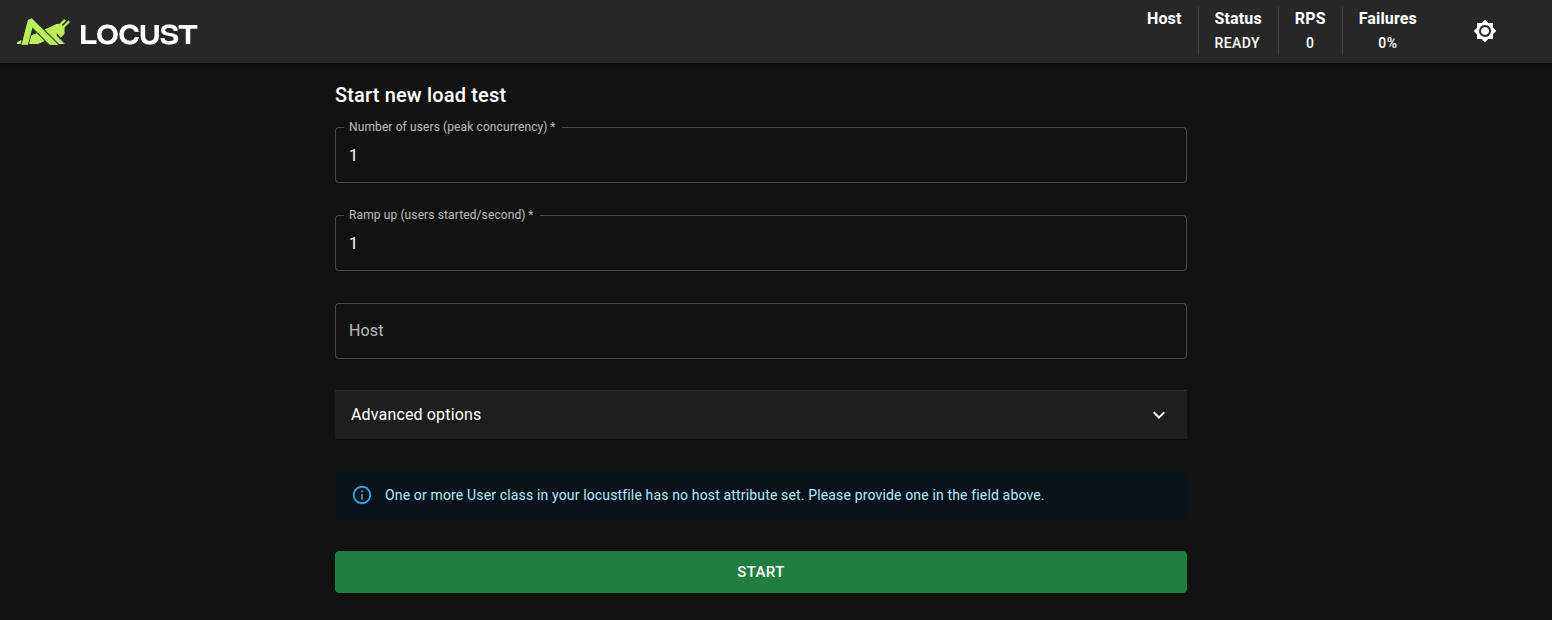
\includegraphics[width=0.9\textwidth]{figures/locust_home.png}
    \caption{Inicio de Locust}
    \label{fig:locust_home}
\end{figure}

En esta interfaz se pueden ajustar los siguientes parámetros:

\begin{itemize}
    \item \textbf{Número de usuarios:} establece cuántos usuarios concurrentes van a realizar la ejecución de la tarea establecida en el script.
    \item \textbf{Ramp up:} establece el tiempo en segundos en el que se van a ir añadiendo los usuarios de manera progresiva.
    \item \textbf{Host:} indica a sobre qué dominio se van a realizar las peticiones.
\end{itemize}

Se empezó ejecuntado el script de login para 100 usuarios y un \textit{ramp up} de 10, de manera que cada 10 segundos, se iban a ir añadiendo usuarios de forma progresiva
hasta llegar a un límite de 100.

Los resultados obtenidos fueron los siguientes:

\begin{figure}[H]
    \centering
    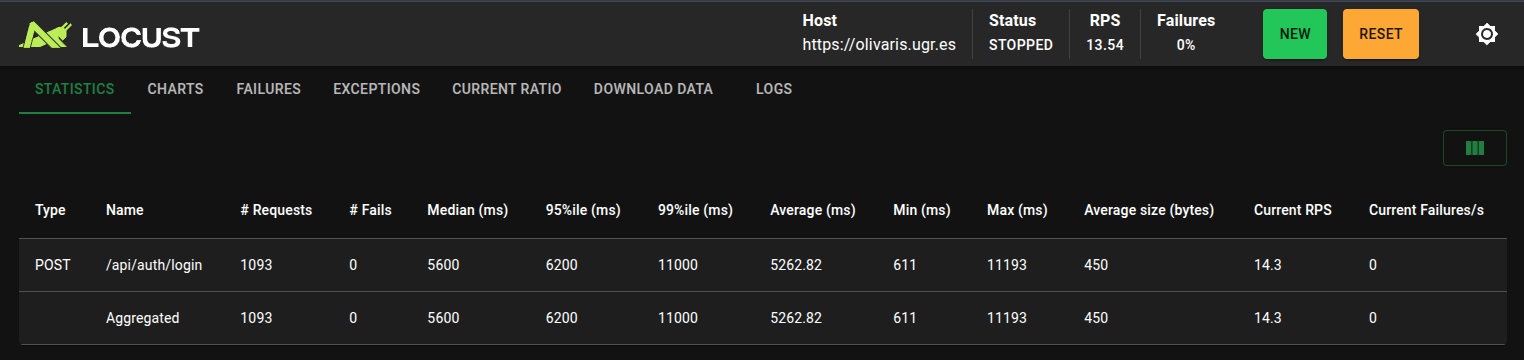
\includegraphics[width=0.9\textwidth]{figures/statistics_100_login_csirc.png}
    \caption{Estadísticas para 100 usuarios en el login desde el CSIRC}
    \label{fig:statistics_100_login_csirc}
\end{figure}

Con estos datos obtenidos se interpreta lo siguiente:

\begin{itemize}
    \item \textbf{Request y failures:} el sistema ha procesado 1093 peticiones de login y no ha habido ningún error. Esto quiere decir que todas las respuestas tenían un código 201
    y que todas ellas contenían el \textit{accessToken} entre sus campos.

    \item \textbf{Median:} indica que el tiempo de respuesta de media es de 5.2 segundos, siendo un tiempo muy alto para una operación de inicio de sesión.
    
    \item \textbf{95\%ile:} esto indica que el 95\% de las peticiones tardaron menos de 6.2 segundos en resolverse. Este dato indica que en general es estable el sistema debido a que
    no hay mucha variabilidad aunque el tiempo sea alto.

    \item \textbf{99\%ile:} indica que el 99\% de las peticiones tardaron menos de 11 segundos. 
    
    \item \textbf{Min y Max:} estos datos indican el tiempo mínimo o más rápido de una petición (611ms) y el tiempo más alto o más lento en procesar una petición (11s).
    
    \item \textbf{RPS:} indica el número de peticiones que el backend está procesando o ``soportando'' por segundo, es decir, procesa 14 peticiones de login cada segundo.
\end{itemize}

Como se puede observar, tiempos de respuesta de 5 segundos aproximadamente para una operación de login con 100 usuarios es demasiado alto. Estos resultados se obtuvieron ejecutando
el sistema desde un servidor proporcionado por el CSIRC, por lo que se pasó a probarlo en local y descartar posibles errores en la arquitectura del sistema, en \textit{querys} a la 
base de datos o en el código.

Ejecutando el mismo script con los mismo datos de usuarios y ramp up pero en localhost, se obtuvieron los siguientes resultados:

\begin{figure}[H]
    \centering
    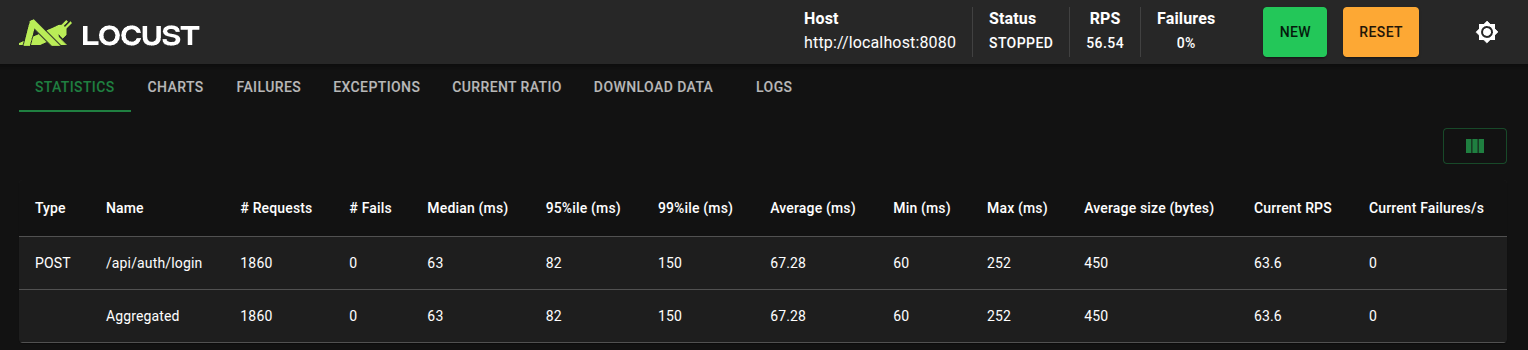
\includegraphics[width=0.9\textwidth]{figures/statis_100_login_local.png}
    \caption{Estadísticas para 100 usuarios en el login desde localhost}
    \label{fig:statis_100_login_local}
\end{figure}

En esta imagen se pueden apreciar resultados más lógicos para un login. Es cierto que es sobre mi PC en local, por lo que no hay una gran latencia pero los resultados se acercan más a
la realidad.

Una vez comprobado que los tiempos son más razonables en local, se hizo la misma prueba pero desplegando el sistema en otro servidor \textit{on-premise} proporcionado por el Juan Luis Laredo,
tutor del presente Trabajo de Fin de Grado. Al ejecutar en este servidor el script con los mismos parámetros se obtuvieron los siguientes resultados:

\begin{figure}[H]
    \centering
    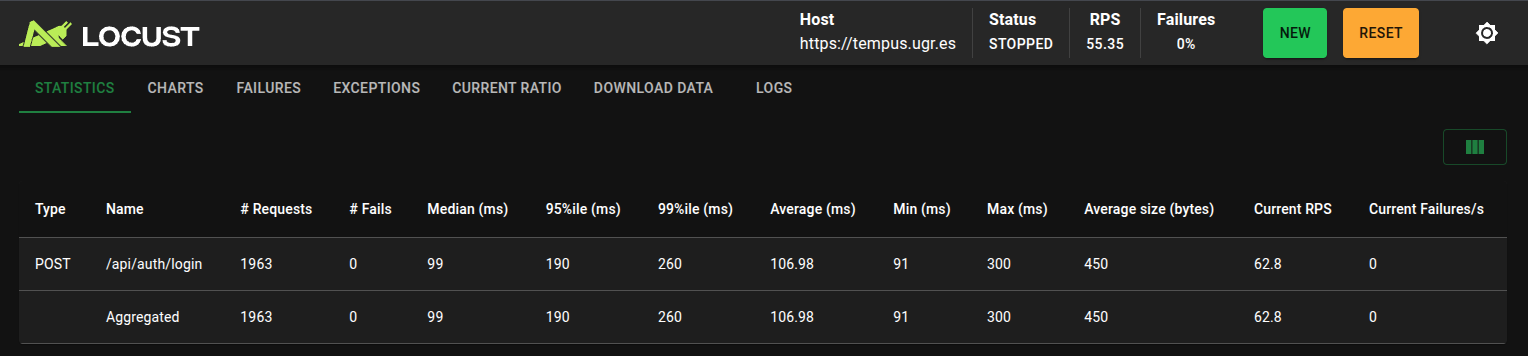
\includegraphics[width=0.9\textwidth]{figures/statis_100_login_tempus.png}
    \caption{Estadísticas para 100 usuarios en el login desde on premise}
    \label{fig:statis_100_login_tempus}
\end{figure}

En este servidor se puede observar como los datos obtenidos son también más razonables para un login con 100 usuarios, ya que se tienen tiempos de respuesta que no llegan a 1 segundo.

Con estas pruebas realizadas tanto en local como con un servidor \textit{on premise}, se descartó la hipótesis de fallos en arquitectura o en código y se dedujo que el servidor del CSIRC
tiene unas prestaciones más reducidas, causando de esta manera tiempos de respuesta bastante más altos que en otras infraestructuras.

\subsection{Comparación de tiempos en el servidor on premise}

A continuación, se va a proceder a ejecutar el script del login en el servidor \textit{on premise} bajo dos condiciones distintas: en una se tendrá 1000 usuarios con un ramp up de 10s, y en otra
se tendrán también 1000 usuarios pero con un ramp up de 100s. Con estos datos se busca ``estresar'' el servidor para ver hasta qué punto puede atender peticiones bajo tiempos de respuesta razonables.

Los resultados con 1000 usuarios y ramp up de 10s son los siguientes:

\begin{figure}[H]
    \centering
    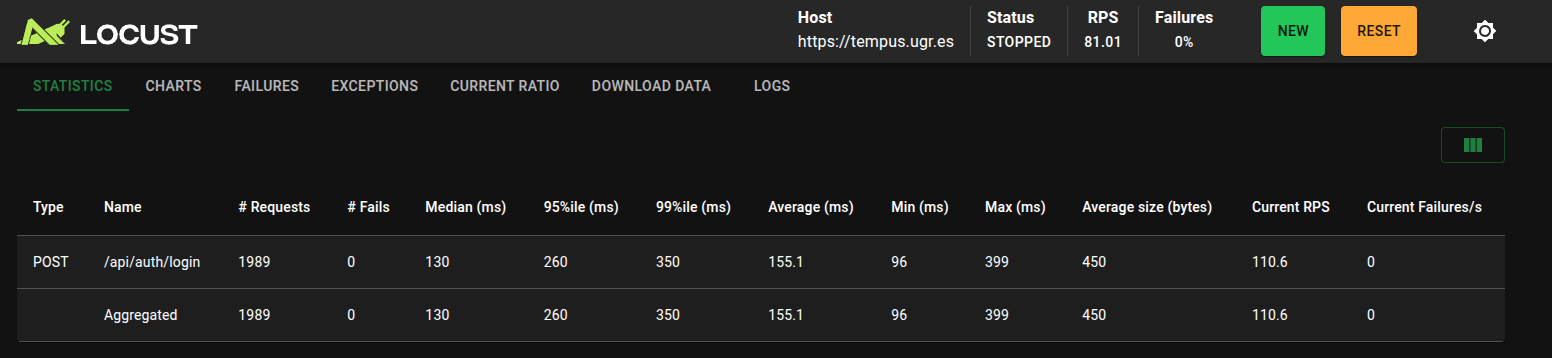
\includegraphics[width=0.9\textwidth]{figures/statis_1000_10_login_tempus.png}
    \caption{Estadísticas para 1000 usuarios en el login desde on premise}
    \label{fig:statis_1000_10_login_tempus}
\end{figure}


Sin embargo, los resultados con 1000 usuarios y ramp up de 100s son los siguientes:

\begin{figure}[H]
    \centering
    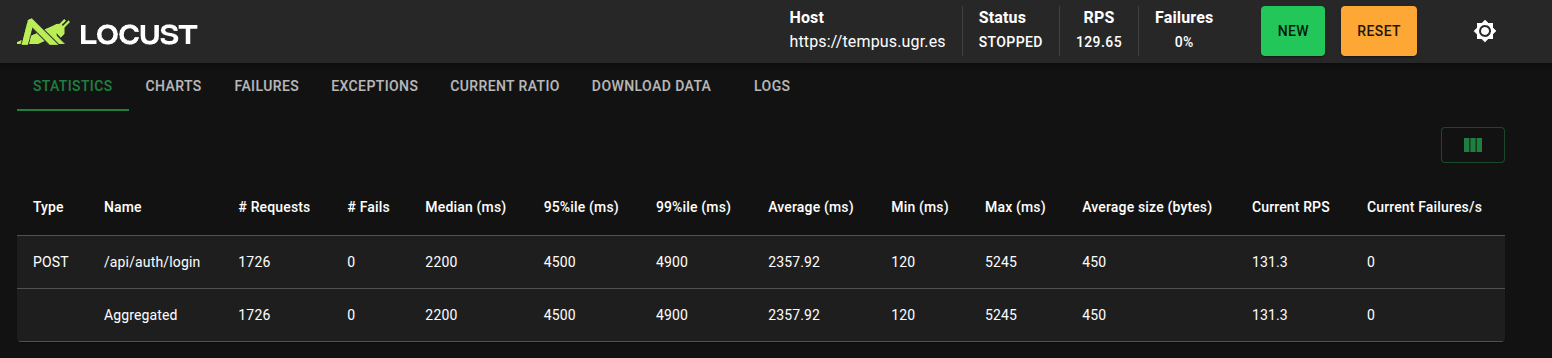
\includegraphics[width=0.9\textwidth]{figures/statis_1000_100_login_tempus.png}
    \caption{Estadísticas para 1000 usuarios en el login desde on premise}
    \label{fig:statis_1000_100_login_tempus}
\end{figure}

Aquí se puede observar como inyectando usuarios cada 100s, los tiempos de respuesta van aumentando llegando hasta los 2 segundos con 1700 peticiones aproximadamente. En este punto, el servidor 
empieza a tener dificultades en procesar las peticiones de inicio de sesión, ya que sigue manteniendo unas RPS aproximadas a las anteriores y siguen entrando más usuarios. Sin embargo,
al tener un ramp up más alto, el servidor está llegando a las máximas peticiones que puede atender, provocando que muchas de ellas se vayan a la cola del servidor y causando
un aumento de la latencia.

Además, otro dato relevador es el percentil 95: en la primera prueba se tiene que el 95\% de las peticiones son ejecutadas en menos de 260ms, mientras que en la segunda prueba, el 95\% de las peticiones
son ejecutadas en menos de 4.5s, lo que indica hay muchas peticiones en cola esperando ser atendidas.

A continuación se va a probar el srcipt que obtiene las parcelas de un usuario con 1000 usuarios y ramp up de 10s. Los resultados obtenidos son los siguientes:

\begin{figure}[H]
    \centering
    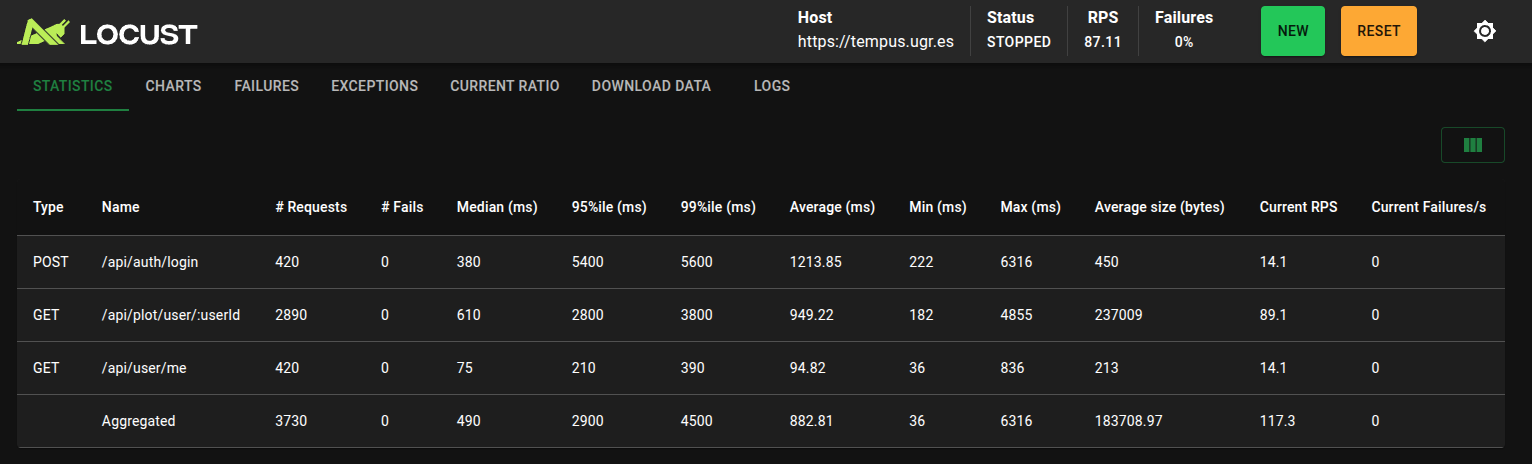
\includegraphics[width=0.9\textwidth]{figures/statis_1000_10_plots_tempus.png}
    \caption{Estadísticas para 1000 usuarios en la obtención de parcelas}
    \label{fig:statis_1000_10_plots_tempus}
\end{figure}

En este caso, se están realizando peticiones a 3 endpoints diferentes, pudiendo observar como el endpoint que obtiene todas las parcelas del usuario tiene los tiempos de respuesta más altos, pero sin
embargo, la gran mayoría de peticiones al endpoint del login tardan más en ser atendidas (95\% en 5s), causado probablemente por una cola saturada de peticiones.



    
    \chapter{Conclusiones y trabajo futuro}

El objetivo principal de este Trabajo de Fin de Grado ha consistido en diseñar e implementar una plataforma digital para la gestión colaborativa de explotaciones de olivar. El 
trabajo parte de la necesidad de organizar de forma estructurada la información asociada a parcelas, recintos, usuarios, entidades habilitadas y actividades agrícolas, en un 
contexto en el que la digitalización y la trazabilidad de la información agraria adquieren cada vez más importancia.

Como respuesta a esta problemática se ha desarrollado Olivaris, un prototipo funcional basado en una arquitectura cliente-servidor. El sistema incorpora un backend con API REST, 
autenticación mediante JWT, control de acceso por roles, gestión de usuarios y entidades, registro de parcelas y recintos, gestión de actividades agrícolas y soporte para información 
geoespacial. Además, se ha desarrollado una aplicación móvil que permite interactuar con las principales funcionalidades del sistema.

Los resultados obtenidos permiten concluir que la solución propuesta es técnicamente viable. Olivaris permite centralizar información relevante de una explotación agrícola, organizarla 
en torno a parcelas y actividades, y gestionar distintos perfiles de usuario con permisos diferenciados. De este modo, el sistema ofrece una base funcional para mejorar la organización 
de la información y facilitar la colaboración entre agricultores y entidades habilitadas.

Uno de los aspectos más relevantes del proyecto es la integración de distintos componentes tecnológicos en una solución coherente: backend, base de datos, información geoespacial, aplicación
móvil, mecanismos de seguridad, despliegue mediante contenedores y pruebas de rendimiento. Esta combinación permite que el sistema no se limite a una funcionalidad aislada, sino que constituya 
una base extensible sobre la que incorporar nuevas capacidades.

Asimismo, el diseño del sistema se ha planteado teniendo en cuenta el marco SIEX/REA/CUE, de forma que la estructura de la información pueda facilitar una posible adaptación futura a los requisitos 
de estas plataformas. Aunque no se ha implementado una integración efectiva con servicios oficiales, el trabajo realizado permite avanzar hacia una gestión agrícola más digital, estructurada y preparada 
para escenarios de interoperabilidad.

Las pruebas realizadas han permitido validar el comportamiento técnico del sistema en distintos escenarios de carga. Aunque esta evaluación no sustituye a una validación completa con usuarios reales, sí 
aporta una primera evidencia sobre el funcionamiento del backend y sobre la influencia que tiene la infraestructura de despliegue en el rendimiento de la aplicación.

En conjunto, Olivaris cumple los objetivos principales planteados al inicio del proyecto y demuestra que es posible construir una plataforma funcional para la gestión colaborativa del olivar utilizando 
tecnologías actuales, abiertas y extensibles.

\section{Limitaciones del sistema}

A pesar de los resultados obtenidos, el sistema presenta algunas limitaciones que deben tenerse en cuenta.

En primer lugar, la plataforma no incorpora todavía una integración efectiva con los servicios oficiales asociados al marco SIEX/REA/CUE. El diseño se ha orientado a facilitar una posible compatibilidad 
futura, pero la conexión real con dichas plataformas queda fuera del alcance implementado.

En segundo lugar, la aplicación no dispone de funcionamiento offline. Esta limitación es relevante en el contexto agrícola, ya que muchas parcelas pueden encontrarse en zonas con conectividad limitada. 
En el estado actual, el uso de la aplicación depende de la conexión con el backend.

Otra limitación es que la generación de informes se encuentra en una fase inicial. Aunque permite generarlos en base a las actividades realizadas, en una herramienta de este tipo sería útil poder generar 
informes en base a los criterios: parcela, campaña, producto aplicado o fecha.

Asimismo, el sistema se ha centrado principalmente en una aplicación móvil. Una versión web permitiría mejorar la consulta, revisión y administración de datos desde ordenador, especialmente para entidades 
habilitadas o usuarios que gestionen un número elevado de parcelas.

Finalmente, la evaluación se ha centrado en pruebas técnicas y de rendimiento. Sería necesario realizar pruebas con usuarios reales del sector agrícola para valorar la usabilidad de la aplicación, la claridad 
de los formularios y la adecuación de los flujos de trabajo a situaciones reales.

\section{Trabajo futuro}

A partir de las limitaciones identificadas, se plantean varias líneas de trabajo futuro.

Una de las más relevantes sería avanzar en la integración con el marco SIEX/REA/CUE, estudiando los formatos de intercambio de información, los requisitos técnicos y los mecanismos de autenticación necesarios 
para una futura conexión con servicios oficiales.

También resultaría importante incorporar funcionamiento offline y sincronización posterior, de forma que el usuario pueda registrar actividades en campo aunque no disponga de conexión en ese momento.

Otra línea de mejora sería ampliar la generación de informes, permitiendo filtrar y exportar información por parcela, campaña, producto aplicado, tipo de actividad o intervalo temporal. Esta funcionalidad aumentaría 
notablemente el valor práctico de la plataforma.

Además, sería conveniente desarrollar una interfaz web que complemente a la aplicación móvil. Esto permitiría ofrecer una experiencia más cómoda para tareas de revisión, administración, generación de informes y gestión 
de grandes volúmenes de información.

Por último, sería interesante realizar pruebas de usabilidad con agricultores, técnicos agrícolas o personal de cooperativas. Esta validación permitiría detectar problemas reales de uso, simplificar formularios y priorizar 
mejor las funcionalidades futuras.

\section{Conclusión final}

Olivaris ha permitido demostrar la viabilidad de una plataforma digital para la gestión colaborativa del olivar, integrando en una misma solución la gestión de usuarios, entidades, parcelas, recintos, actividades agrícolas, 
información geoespacial y control de permisos.

Aunque el sistema presenta limitaciones y todavía existen funcionalidades por desarrollar, el trabajo realizado constituye una base sólida y extensible. En este sentido, el TFG cumple su objetivo principal: construir un prototipo 
funcional y técnicamente coherente que contribuye a la digitalización de la gestión agrícola y que puede servir como punto de partida para futuras evoluciones hacia una herramienta más completa y cercana a las necesidades del sector.

    \chapter*{Anexo 1: Declaración de uso responsable de herramientas de IA}
\addcontentsline{toc}{chapter}{Anexo 1: Declaración de uso responsable de herramientas de IA}

Durante la elaboración de este Trabajo de Fin de Grado se han utilizado herramientas de inteligencia artificial generativa, como modelos de lenguaje de gran escala
y asistentes de programación, de forma auxiliar y bajo criterios de uso ético, crítico y responsable.

El uso de estas herramientas ha estado orientado a apoyar determinadas tareas del proceso de desarrollo del proyecto, sin sustituir la auditoría personal, el criterio
técnico en la toma de decisiones y la responsabilidad acádemica del estudiante. 

En particular, las herramientas de IA se han utilizado para las siguientes finalidades:

\begin{itemize}
    \item Revisión lingüística, mejora de estilo y reformulación de fragmentos redactados previamente por el estudiante.
    \item Generación de ejemplos, explicaciones alternativas o aclaraciones conceptuales.
    \item Apoyo en la depuración, optimización y refactorización del código desarrollado.
    \item Generación de fragmentos de código auxiliares posteriormente revisados, adaptados y validados de acuerdo al criterio del estudiante.
\end{itemize}

En todos los casos expuestos anteriormente, los resultados proporcionados han sido revisados críticamente. El estudiante ha comprobado la corrección técnica, la coherencia
con los objetivos del trabajo, la adecuación al contexto académico y, cuando ha sido necesario, la validez de los algoritmos y fragmentos de código generados.

El uso de IA generativa no ha sustituido el trabajo intelectual propio ni la toma de decisiones fundamentales del proyecto. El diseño, desarrollo, análisis, evaluación, 
redacción final y conclusiones del TFG son responsabilidad del autor de este trabajo.

El estudiante declara que ha utilizado estas herramientas de forma honesta y transparente, evitando presentar como propio trabajo no comprendido, no revisado o generado
automáticamente sin supervisión crítica.

Teniendo esto en cuenta, las herramientas utilizadas han sido: 

\begin{itemize}
    \item \textbf{ChatGPT y Gemini:} utilizados para mejorar la redacción de distintas partes de la memoria, buscando una mayor coherencia y estilo língüístico. También han sido
    utilizados para realizar consultas a nivel técnico sobre cómo utilizar ciertas herramientas (como Locust o Docker), o cómo realizar la conexión entre los componentes.
    
    \item \textbf{Github Copilot:} ha sido utilizado para la generación de fragmentos de código del frontend principalmente, buscando dar una mejora de la usabilidad de la aplicación
    así como del apartado visual. También, ha sido utilizado para optimizar partes del código del despliegue con Docker.
\end{itemize}
    
    % Anexos

    %% Anexo : Glosario 
    \chapter*{Anexo: Glosario}

En esta sección se van a recoger las definiciones de términos que hayan sido utilizados en la memoria:

\begin{description}
    \item[\hypertarget{api}{Application Programming Interface (API)}]: conjunto de reglas, protocolos y herramientas 
    que permite que dos aplicaciones de software se comuniquen e intercambien datos entre sí de forma segura.
    
    \item[\hypertarget{singlePageApplication}{Single Page Application}]: es un tipo de aplicación web que ejecuta todo 
    su contenido en una sola página, cargando el contenido HTML, CSS y JavaScript por completo al abrir la web. Al ir
    pasando de una sección a otra, solo necesita cargar el contenido nuevo de forma dinámica si este lo requiere, 
    pero no hace falta cargar la página por completo.

    \item[\hypertarget{progressiveWebApps}{Progressive Web Apps}]: es una aplicación web que, gracias a tecnologías 
    modernas (HTML, JavaScript, CSS), ofrece una experiencia similar a una aplicación nativa, permitiendo su 
    instalación en la pantalla de inicio, funcionar sin conexión y enviar notificaciones push, todo desde una única 
    base de código y sin necesidad de tiendas de aplicaciones, combinando lo mejor de la web y las apps nativas. 

    \item[\hypertarget{clientSideRendering}{Client-Side Rendering}]: técnica que permite al navegador del usuario 
    descargar un HTML mínimo y luego usar JavaScript para construir y renderizar el contenido de la página web 
    dinámicamente en el cliente.

    \item[\hypertarget{marcosTrabajo}{Marcos de trabajo (\textit{frameworks})}]: conjunto estandarizado de herramientas, 
    librerías, reglas y componentes reutilizables que actúa como esqueleto para desarrollar software, aplicaciones web 
    o móviles de forma rápida y eficiente.

    \item[\hypertarget{jwt}{JSON Web Token}]: es un estándar abierto para la transmisión segura de la información entre dos partes 
    (típicamente un cliente y un servidor). Cada JWT es firmado digitalmente para prevenir su manipulación y además, contiene 
    \textit{claims} (piezas de información) sobre el usuario o la sesión.

    \item[\hypertarget{singleSignOn}{Single Sign-on}]: procedimiento de autenticación que habilita a un usuario determinado para 
    acceder a varios sistemas con una sola instancia de identificación.

    \item[\hypertarget{jsonb}{JSONB}]: formato binario para guardar JSON que permite indexar los datos.
\end{description}

    % Bibliografía
    \bibliographystyle{unsrtnat}
    \nocite{*}
    \bibliography{bibliografia.bib}
        

% Fin del documento
\end{document}